%%
%% This is file `ubcsample.tex',
%% generated with the docstrip utility.
%
% The original source files were:
%
% ubcthesis.dtx  (with options: `ubcsampletex')
%% 
%% This file was generated from the ubcthesis package.
%% --------------------------------------------------------------
%% 
%% Copyright (C) 2001
%% Michael McNeil Forbes
%% mforbes@alum.mit.edu
%% 
%% This file may be distributed and/or modified under the
%% conditions of the LaTeX Project Public License, either version 1.2
%% of this license or (at your option) any later version.
%% The latest version of this license is in
%%    http://www.latex-project.org/lppl.txt
%% and version 1.2 or later is part of all distributions of LaTeX
%% version 1999/12/01 or later.
%% 
%% This program is distributed in the hope that it will be useful,
%% but WITHOUT ANY WARRANTY; without even the implied warranty of
%% MERCHANTABILITY or FITNESS FOR A PARTICULAR PURPOSE.  See the
%% LaTeX Project Public License for more details.
%% 
%% This program consists of the files ubcthesis.dtx, ubcthesis.ins, and
%% the sample figures fig.eps and fig.fig.
%% 
%% This file may be modified and used as a base for your thesis without
%% including the licence agreement as long as the content (i.e. textual
%% body) of the file is completely rewritten. You must, however, change
%% the name of the file.
%% 
%% This file may only be distributed together with a copy of this
%% program. You may, however, distribute this program without generated
%% files such as this one.
%% 

% This Sample thesis requires \LaTeX2e
\NeedsTeXFormat{LaTeX2e}[1995/12/01]
\ProvidesFile{ubcsample.tex}[2015/05/31 v1.72 ^^J
 University of British Columbia Sample Thesis]
% This is the \documentclass[]{} command.  The manditory argument
% specifies the "flavour" of thesis (ubcthesis for UBC).  The
% optional arguments (in []) specify options that affect how the
% thesis is displayed.  Please see the ubcthesis documentation for
% details about the options.
\documentclass[msc,oneside]{ubcthesis}
%
% To compile this sample thesis, issue the following commands:
% latex ubcsample
% bibtex ubcsample
% latex ubcsample
% latex ubcsample
% latex ubcsample
%
% To view use xdvi (on unix systems):
% xdvi ubcsample.dvi
%
% To make a postscript file, use dvips:
% dvips -o ubcsample.ps ubcsample.dvi
%
% To view the postscript file, use ghostview or gv (on unix systems):
% gv ubcsample.ps
%
%************************************************
% Optional packages.
%
% The use of these packages is optional, but they provide various
% tools for more flexible formating.  The sample thesis uses these,
% but if you remove the example code, you should be able to exclude
% these packages.  Only standard packages have been described here;
% they should be installed with any complete LaTeX instalation, but
% if not, you can find them at the Comprehensive TeX Archive Network
% (CTAN): http://www.ctan.org/
%

%******** afterpage ***************************
% This package allows you to issue commands at the end of the current
% page.  A good use for this is to use the command
% \afterpage{\clearpage} right after a figure.  This will cause the
% figure to be inserted on the page following the current one (or on
% the current page if it will fit) but will not break the page in the
% middle.
\usepackage{afterpage}

%******** float *********************************
% This package allows you to customize the style of
% "floats"---floating objects such as figures and tables.  In
% addition, it allows you to define additional floating objects which
% may be included in a list similar to that produces by \listoftables
% and \listoffigures.  Common uses include introducing floats for
% programs and other code bits in Compute Science and Chemical Schema.
\usepackage{float}

%******** tocloft *******************************
% This package allows you to customize and define custom lists such
% as a list of programs or Chemical Scheme.  Note: if you use the
% subfigure package, you must specify that you do as an option here.
% The title option uses the default formatting.  We do not use this
% here as the default formatting is acceptable.  Use the float
% package instead unless you need the extra formatting control
% provided by tocloft.
%\usepackage[subfigure, titles]{tocloft}

%******** alltt *********************************
% The alltt package allows you to include files and have them
% formatted in a verbatim fashion.  This is useful for including
% source code from an additional file.
%\usepackage{alltt}

%******** listings ******************************
% The listings package may be used to include chunks of source code
% and has facilities for pretty-printing many languages.
%\usepackage{listings}

%******** longtable *****************************
% The longtable package allows you to define tables that span
% multiple pages.
\usepackage{longtable}

%******** graphics and graphicx *****************
% This allows you to include encapsulated postscript files.  If you
% don't have this, comment the \includegraphics{} line following the
% comment "%includegraphics" later in this file.
\usepackage{graphicx}

%******** subfigure *****************************
% The subfigure package allows you to include multiple figures and
% captions within a single figure environment.
%\usepackage{subfigure}

%******** here **********************************
% The here package gives you more control over the placement of
% figures and tables.  In particular, you can specify the placement
% "H" which means "Put the figure here" rather than [h] which means
% "I would suggest that you put the figure here if you think it looks
% good."
%\usepackage{here}

%******** pdflscape ********************************
% This allows you to include landscape layout pages by using the
% |landscape| environment.  The use of |pdflscape| is preferred over
% the standard |lscape| package because it automatically rotates the
% page in the pdf file for easier reading.  (Thanks to Joseph Shea
% for pointing this out.)
\usepackage{pdflscape}

%******** natbib ********************************
% This is a very nice package for bibliographies.  It includes options
% for sorting and compressing bibliographic entries.
\usepackage[numbers,sort&compress]{natbib}

%******** psfrag ******************************
% This allows you to replace text in postscript pictures with formated
% latex text.  This allows you to use math in graph labels
% etc. Uncomment the psfrag lines following the "%psfrag" comment
% later in this file if you don't have this package.  The replacements
% will only be visible in the final postscript file: they will be
% listed in the .dvi file but not performed.
\usepackage{psfrag}

%******** hyperref *****************************
% Please read the manual:
% http://www.tug.org/applications/hyperref/manual.html
%
% This adds hyperlinks to your document: with the right viewers (later
% versions of xdvi, acrobat with pdftex, latex2html etc.) this will
% make your equation, figure, citation references etc. hyperlinks so
% that you can click on them.  Also, your table of contents will be
% able to take you to the appropriate sections.  In the viewers that
% support this, the links often appear with an underscore.  This
% underscore will not appear in printed versions.
%
% Note: if you do not use the hypertex option, then the dvips driver
% may be loaded by default.  This will cause the entries in the list
% of figures and list of tables to be on a single line because dvips
% does not deal with hyperlinks on broken lines properly.
%
% NOTE: HYPERREF is sensitive to the ORDER in which it is LOADED.
% For example, it must be loaded AFTER natbib but BEFORE newly
% defined float environments.  See the README file with the hyperref
% for some help with this.  If you have some very obscure errors, try
% first disabling hyperref.  If that fixes the problem, try various
% orderings.
%
% Note also that there is a bug with versions before 2003/11/30
% v6.74m that cause the float package to not function correctly.
% Please ensure you have a current version of this package.  A
% warning will be issued if you leave the date below but do not have
% a current version installed.
%
% Some notes on options: depending on how you build your files, you
% may need to choose the appropriate option (such as [pdftex]) for the
% backend driver (see the hyperref manual for a complete list).  Also,
% the default here is to make links from the page numbers in the table
% of contents and lists of figures etc.  There are other options:
% excluding the [linktocpage] option will make the entire text a
% hyperref, but for some backends will prevent the text from wrapping
% which can look terrible.  There is a [breaklinks=true] option that
% will be set if the backend supports (dvipdfm for example supports
% it but does not work with psfrag.)
%
% Finally, there are many options for choosing the colours of the
% links.  These will be included by default in future versions but
% you should probably consider changing some now for the electronic
% version of your thesis.
\usepackage[unicode=true,
  linktocpage,
  linkbordercolor={0.5 0.5 1},
  citebordercolor={0.5 1 0.5},
  linkcolor=blue]{hyperref}

% If you would like to compile this sample thesis without the
% hyperref package, then you will need to comment out the previous
% \usepackage command and uncomment the following command which will
% put the URL's in a typewriter font but not link them.
%\newcommand\url[1]{\texttt{#1}}

%******** setspace *******************************
% The setspace package allows you to manually set the spacing of the
% file.  UBC may require 1.5 spacing for microfilming of theses.  In
% this case you may obtain this by including this package and issuing
% one of the following commands:
%\usepackage{setspace}
%\singlespacing
%\onehalfspacing
%\doublespacing







\usepackage{caption}
\usepackage{amsmath}
\usepackage{amsthm}
\usepackage{bbm}
\usepackage{tikz}
\usepackage[title]{appendix}
%\usepackage{hyperref}
\usetikzlibrary{patterns}
%\usepackage{stix}
\usepackage{amssymb}
\usepackage{enumitem}


\newtheorem{theorem}{Theorem}
\newtheorem{corollary}{Corollary}
\newtheorem{lemma}{Lemma}
\newtheorem{proposition}{Proposition}
\newtheorem{assumption}{Assumption}
 
\newcommand{\C}{\mathbb{C}}
%\newcommand{\H}{\mathcal{H}}
\newcommand{\Tr}{\text{Tr}}
\newcommand{\tr}{\text{tr}}
\newcommand{\eps}{\varepsilon}
\newcommand{\R}{\mathbb{R}}
\newcommand{\N}{\mathbb{N}}
\newcommand{\Z}{\mathbb{Z}}
\newcommand{\norm}[1]{\lVert #1 \rVert}
\newcommand{\One}{\mathbbm{1}}
\newcommand{\Var}{\text{Var}}
\newcommand{\F}{\mathcal{F}}
\newcommand{\G}{\mathcal{G}}
\newcommand{\U}{\mathcal{U}}







% These commands are optional.  The defaults are shown.  You only
% need to include them if you need a different value
\institution{The University Of British Columbia}

% If you are at the Okanagan campus, then you should specify these
% instead.
%\faculty{The College of Graduate Studies}
%\institutionaddress{Okanagan}
\faculty{The Faculty of Graduate Studies}
\institutionaddress{Vancouver}

% You can issue as many of these as you have...
\previousdegree{B.Sc. Hons, The University of New Brunswick, 2019}

% You can override the option setting here.
% \degreetitle{Jack of All Trades}

% These commands are required.
\title{The Quantum Hall Effect and Bulk-Edge Correspondence on Lattice Systems}
%\subtitle{With a Subtitle}
\author{Justin Furlotte}
\copyrightyear{2022}
\submitdate{\monthname\ \number\year} % The "\ " is required after
                                      % \monthname to prevent the
                                      % command from eating the space.
\program{Mathematics}

% These commands are presently not required for UBC theses as the
% advisor's name and title are not presently required anywhere.
%\advisor{Ariel R.~Zhitnitsky}
%\advisortitle{Professor of Physics}

% One might want to override the format of the section and chapter
% numbers.  This shows you how to do it.  Note that the current
% format is acceptable for submission to the FoGS: If you wish to modify
% these, you should check with the FoGS explicity. prior to making
% the modifications.
\renewcommand\thepart         {\Roman{part}}
\renewcommand\thechapter      {\arabic{chapter}}
\renewcommand\thesection      {\thechapter.\arabic{section}}
\renewcommand\thesubsection   {\thesection.\arabic{subsection}}
\renewcommand\thesubsubsection{\thesubsection.\arabic{subsubsection}}
\renewcommand\theparagraph    {\thesubsubsection.\arabic{paragraph}}
\renewcommand\thesubparagraph {\theparagraph.\arabic{subparagraph}}

\setcounter{tocdepth}{2}
\setcounter{secnumdepth}{2}

% Here is an example of a "Program" environment defined with the
% "float" package.  The list of programs will be stored in the file
% ubcsample.lop and the numbering will start with the chapter
% number.  The style will be "ruled".
\floatstyle{ruled}
\newfloat{Program}{htbp}{lop}[chapter]

% Here is the start of the document.
\begin{document}

\graphicspath{ {c:/user/justin/grad school/Thesis Git/ubc thesis} }


%% This starts numbering in Roman numerals as required for the thesis
%% style and is mandatory.
\frontmatter

%%% The order of the following components should be preserved.  The order
%%% listed here is the order currently required by FoGS:        \\
%%% Title (Mandatory)                                           \\
%%% Preface (Manditory if any collaborator contributions)       \\
%%% Abstract (Mandatory)                                        \\
%%% List of Contents, Tables, Figures, etc. (As appropriate)    \\
%%% Acknowledgements (Optional)                                 \\
%%% Dedication (Optional)                                       \\

\maketitle                      %% Mandatory
\begin{abstract}                %% Mandatory -  maximum 350 words
  The \texttt{genthesis.cls} \LaTeX{} class file and accompanying
  documents, such as this sample thesis, are distributed in the hope
  that it will be useful but without any warranty (without even the
  implied warranty of fitness for a particular purpose).  For a
  description of this file's purpose, and instructions on its use, see
  below.

  These files are distributed under the GPL which should be included
  here in the future.  Please let the author know of any changes or
  improvements that should be made.

  Michael Forbes.
  mforbes@physics.ubc.ca
\end{abstract}

\chapter{Preface} % Manditory if any of the conditions are met

You must include a preface if any part of your research was partly or
wholly published in articles, was part of a collaboration, or required
the approval of UBC Research Ethics Boards.

The Preface must include the following:

\begin{itemize}
\item A statement indicating the relative contributions of all
  collaborators and co-authors of publications (if any), emphasizing
  details of your contribution, and stating the proportion of research
  and writing conducted by you.
\item A list of any publications arising from work presented in the
  dissertation, and the chapter(s) in which the work is located.
\item The name of the particular UBC Research Ethics Board, and the
  Certificate Number(s) of the Ethics Certificate(s) obtained, if
  ethics approval was required for the research.
\end{itemize}

%%% Sections and subsections etc. in the Preface should in general
%%% not be listed in the table of contents, so use the starred form
%%% of \section etc.
\section*{Examples}
Chapter~\ref{cha:apple_ref} is based on work conducted in UBC's Maple
Syrup Laboratory by Dr. A.  Apple, Professor B. Boat, and Michael
McNeil Forbes. I was responsible for tapping the trees in forests X
and Z, conducted and supervised all boiling operations, and performed
frequent quality control tests on the product.

A version of chapter~\ref{cha:apple_ref} has been
published~\cite{Apple:2010}. I conducted all the testing and wrote
most of the manuscript. The section on ``Testing Implements'' was
originally drafted by Boat, B.  Check the first pages of this
chapter to see footnotes with similar information.

Note that this preface must come before the table of contents.  Note
also that this section ``Examples'' should not be listed in the table
of contents, so we have used the starred form: \verb|\section*{Example}|.

\tableofcontents                %% Mandatory
\listoftables                   %% Mandatory if thesis has tables
\listoffigures                  %% Mandatory if thesis has figures
\listof{Program}{List of Programs} %% Optional
%% Any other lists should come here, i.e.
%% Abbreviation schemes, definitions, lists of formulae, list of
%% schemes, glossary, list of symbols etc.

\chapter{Acknowledgements}      %% Optional
This is the place to thank professional colleagues and people who have
given you the most help during the course of your graduate work.

\chapter{Dedication} %% Optional
The dedication is usually quite short, and is a personal rather than
an academic recognition.  The \emph{Dedication} does not have to be
titled, but it must appear in the table of contents.  If you want to
skip the chapter title but still enter it into the Table of Contents,
use this command \verb|\chapter[Dedication]{}|.

Note that this section is the last of the preliminary pages (with
lowercase Roman numeral page numbers).  It must be placed
\emph{before} the \verb|\mainmatter| command.  After that, Arabic
numbered pages will begin.

% Any other unusual prefactory material should come here before the
% main body.

% Now regular page numbering begins.
\mainmatter

% Parts are the largest structural units, but are optional.
%\part{Thesis}

% Chapters are the next main unit.
\chapter{This is a Chapter}




\section{Introduction}

\subsection{History}

Since its unexpected discovery in 1980, the Quantum Hall Effect (QHE) has captured significant interest in the mathematical physics community.

\subsection{Heuristic Arguments}

\subsubsection{The Classical Hall Effect}

Using classical electromagnetism is not enough to predict the plateaux seen experimentally. Suppose we have a 2-dimensional electron gas, and let $\vec{B} = B\hat{x_3}$ be a magnetic field piercing the plane of the electrons. They are subjected to a Lorentz force

\[m\dot{\vec{v}} = -q\vec{v}\times\vec{B} .\]

The solution to this differential equation is given by the \emph{cyclotron orbits},

\[\begin{pmatrix} x_1(t)\\x_2(t)\\x_3(t) \end{pmatrix} = \begin{pmatrix} a + r\sin(\omega_Bt+\phi) \\ b + r\cos(\omega_Bt+\phi) \\ 0 \end{pmatrix}\]

where $\omega_B = qB/m$ is the \emph{cylontron frequency}. An electric field $\vec{E}=E\hat{x_1}$ is introduced, and the electrons move in the $x_1$-direction. We now employ the \emph{Drude model},

\[m\dot{\vec{v}} = -q(\vec{E}+\vec{v}\times\vec{B}) + \frac{m}{\tau}\vec{v},\]

where the final term is a linear friction term, and $\tau$ is the scattering time. At equilibrium, the equation reads

\[\vec{J} + \frac{q\tau}{m}\vec{J}\times\vec{B} = -\frac{q^2n\tau}{m}\vec{E},\]

where $\vec{J} = -nq\vec{v}$ is the current density, related to the velocity by the density of electrons per unit area $n$. In matrix notation, this reads

\[\begin{pmatrix} 1 & \omega_B\tau \\ -\omega_B\tau & q \end{pmatrix}\vec{J} = -\frac{q^2n\tau}{m}\vec{E}.\]

Since the matrix on the left is invertible, we may write $\vec{J} = \sigma \vec{E}$, which is Ohm's Law. The \emph{conductivity tensor} is given by

\[\sigma = \begin{pmatrix} \sigma_{xx} & \sigma_{xy} \\ -\sigma_{xy} & \sigma_{yy} \end{pmatrix} = -\frac{q^2n\tau}{m(1+\omega_B^2\tau^2)}\begin{pmatrix} 1 & -\omega_B\tau \\  \omega_B\tau& 1 \end{pmatrix}.\]

The off-diagonal components, $\pm\frac{q^2n\tau}{m(1+\omega_B^2\tau^2)}\omega_B\tau$, are responsible for the Hall effect; the magnetic field induces a component of the current in the $x_2$-direction, in addition to the one in the $x_1$-direction from the electric field. 

When making a measurement, physicists actually measure the resistivity $\rho = \sigma^{-1}$. In particular, the \emph{Hall resistivity} is given by 

\[\rho_{xy} = \frac{B}{nq}.\]

The key prediction of the classical theory is that the Hall resistivity is increases linearly in response to the strength of the magnetic field.

\newpage
\subsubsection{The Quantum Hall Effect}

Von Klitzing's experimental observation in 1980 made it clear that classical electromagnetism is not sufficient to describe the Hall effect. At a temperature of about 8mK, the Hall resistivity looked like this as a function of the magnetic field strength.

\begin{figure}[h!]
\centering
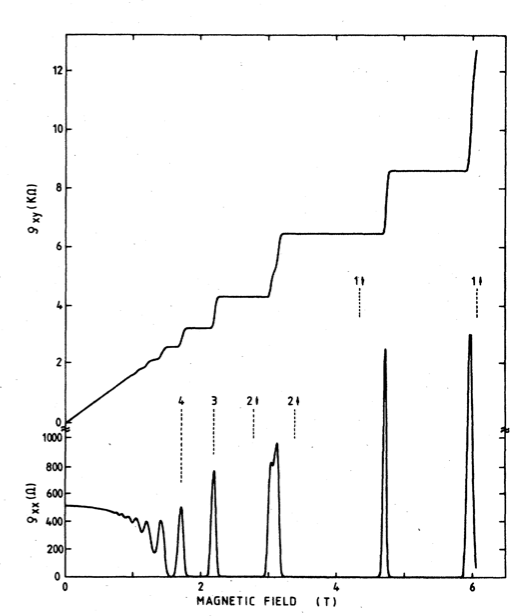
\includegraphics{vonklitzing}
\caption{The Hall resistivity as a function of the magnetic field strength. Distinct plateaux are clearly visible.}
\label{fig:vonklitzing}
\end{figure}

Even more surprising, the plateaux occur at the values

\[\rho_{xy} = \frac{2\pi \hbar}{nq},\]

where $n$ is an integer. In fact, this integer can be measured to such extraordinary precision (to about $3\times10^{-10})$ that as of 2020, the SI definition of the Ohm itself has been redefined in terms of the quantum Hall resistivity.

The first explanation employing quantum mechanics is due to Laughlin in (need to add). 

An intriguing mathematical fact of the quantum Hall effect is the equality of bulk and edge conductivity, in the sense that whether the system is assumed to have an edge or not is immaterial. Proving this fact, both in the interacting and noninteracting setting, is the main focus of this thesis.

\section{Nonnteracting Setting}

Consider the lattice $\Z^2$, and the associated Hilbert space of square-summable sequences of vectors in $\C^n$,

\[\ell^2(\mathbb{Z}^2, \mathbb{C}^n) = \left\{ (x_i)_{i\in\Z^2} \subset \mathbb{C}^n \; : \; \sum_{i \in \Z^2} \norm{x_i}^2 < \infty \right\},\]

with inner product $\langle x, y\rangle = \sum_{i\in\Z^2} x_i\overline{y_i}$. We denote this as $\ell^2(\Z^2)$ for short. On this Hilbert space we define a \emph{bulk Hamiltonian} $H_B:\ell^2(\Z^2)\to\ell^2(\Z^2)$, whose matrix elements follow a short-range assumption:



\begin{assumption}
There exists some $\alpha>0$ such that
\[\sup_{y\in\Z^2}\sum_{x\in\Z^2}|H_B(x,y)|(e^{\alpha|x-y|}-1) \leq C < \infty,\]
where $|x| = |x_1|+|x_2|$ is the taxicab metric.
\label{ass:shortrange}
\end{assumption}

%\[\sigma_B(\lambda) = -i\Tr(P_\lambda[[P_\lambda,\Lambda_1],[P_\lambda,\Lambda_2]])\]

%where $P_\lambda$ is the projection onto the eigenstates of $H_B$ with energy lies in $(-\infty,\lambda)$, and where 

%\[\Lambda_i(x) = \begin{cases} 1 & x_i < 0\\ 0 & x_i \geq 0\end{cases}\]

%are characteristic functions. 

We also construct an \emph{edge Hamiltonian} on the lattice $\Z^2_a := \{x \in \Z^2 : x_2 > -a\}$, denoted by $H_a:\ell^2(\Z^2_a) \to \ell^2(\Z^2_a)$. The bulk and edge Hamiltonians are related by the \emph{edge operator}

\[E_a : \ell^2(\Z^2_a) \to \ell(\Z^2),\]

\[E_a := J_aH_a - H_BJ_a,\]

where $J_a : \ell^2(\Z_a^2) \to \ell(\Z^2)$ denotes extension by zeroes. We require only that that the edge operator satisfies the edge assumption

\begin{assumption}
The edge operator satisfies
\[\sup_{z\in\Z^2}\sum_{y\in\Z^2_a} |E_a(x,y)| e^{\alpha(|x_2 + a| + |x_1-y_1|)} \leq C < \infty\]
for some $\alpha>0$, where $|x| = |x_1|+|x_2|$ is the taxicab metric.
\label{ass:edge}
\end{assumption}




%Each site $x \in \mathbb{Z}^2$ gets an associated Hilbert space $\mathcal{H}_x$; in our setting, we only consider the finite Hilbert spaces $\mathcal{H}_x = \C^{n_x}$. The dimension of these Hilbert spaces is bounded uniformly in $x$. We consider the total Hilbert space $\mathcal{H} = \ell^2(\mathbb{Z}^2)$. For example, one might consider a system of a spin (or multiple spins, in the interacting setting) at the lattice sites, in which case the Hilbert space $\mathcal{H}_x$ at each site would be $\C^2$, and the total Hilbert space $\mathcal{H}$ would be isomorphic to $\otimes_x \mathcal{H}_x$. States would then be the square summable wavefunctions $\mathcal{H} \ni \psi$, $\otimes_x\psi_x \in \otimes_x \mathcal{H}_x$.

%The Hilbert space $\ell^2(\Z^2)$ is the ``bulk" setting, i.e. the setting in which we consider an infinite two-dimensional medium with no edges, and we consider a ``bulk Hamiltonian" $H_B$ on this Hilbert space. We also define the ``edge" Hilbert space $\ell^2(\Z_a^2)$ and an associated ``edge Hamiltonian" $H_a$, where $\Z^2_a := \{(n,m) \in \Z^2 : n \geq -a\}$. The bulk and edge Hamiltonians are related by the edge operator $E_a : \ell^2(\Z^2_a) \to \ell(\Z^2)$ defined by

%\[E_a := J_aH_a - H_BJ_a,\]

%where $J_a : \ell^2(\Z_a^2) \to \ell(\Z^2)$ denotes extension by zeroes. We assume that

%\begin{assumption}
%The edge operator satisfies
%\[\sup_{z\in\Z^2}\sum_{y\in\Z^2_a} |E_a(x,y)| e^{\alpha(|x_2 + a| + |x_1-y_1|)} \leq C < \infty\]
%for some $\alpha>0$, where $|x| = |x_1|+|x_2|$ is the taxicab metric.
%\label{ass:edge}
%\end{assumption}



The interpretation is that $E_a = J_aH_a - H_BJ_a$ is the difference between first applying $H_a$ on $\ell^2(\Z^2_a)$, and then making everything below $-a$ into zeroes, versus first making all $x \in \Z^2$ such that $x_2 < -a$ zeroes, and the applying $H_B$. The assumption ensures that the effects from introducing the edge at $-a$ die exponentially as we move upward away from the edge (due to the $|x_2 - (-a)|$ term in the exponent), and also terms do not interact too much as their $x_1$ distance increases (due to the $|x_1-y_1|$ term in the exponent). 

A simple example of an edge Hamiltonian satisfying the edge condition is $H_a = J_a^*H_BJ_a$, which gives $E_a = (\mathcal{J}_a\mathcal{J}_a^*-1)H_B$. The idea is that for a state $\psi \in \ell^2(\Z^2_a)$, we have $\langle \psi, H_a \psi \rangle = \langle (J_a \psi), H_B (J_a\psi) \rangle$, which we interpret as the edge Hamiltonian having the same expectation as the bulk Hamiltonian if we just transformed all the states with support below the line $x_2=-a$ into zeroes below $x_2=-a$.  The edge operator is 

\[E_a = (J_aJ_a^*-\One)H_BJ_a = \begin{cases} -H_B(x,y) & \text{if } x_2 < -a \\ 0 & \text{if } x_2\geq -a\end{cases}\]

Intuitively, there is no difference between $H_B$ and $H_a$ on $\Z^2_a$. The edge assumption \ref{ass:edge} then follows from the bound $|E_a(x,y)|\leq |H_B(x,y)|$ and the short range assumption \ref{ass:shortrange}.

We also make the following assumption about the bulk Hamiltonian.

\begin{assumption}
The bulk Hamiltonian has a spectral gap. That is, there exists an interval $\Delta \subset \R$ such that for all $L$, 
\[\Delta \cap \emph{Spec}(H_B) = \varnothing.\]
\end{assumption}

\textit{Remark}: The spectral gap assumption can be relaxed to a ``mobility gap" assumption,
\[\sup_{f \in B_c(\Delta)}|f(H_B)(x,y)|(1+|x|)^{-\alpha_1}e^{\alpha_2|x-y|} < \infty\]
for some $\alpha_1>0$, where $B_c(\Delta)$ is the set of Borel functions $f$ which are constant on $(-\infty,\inf \Delta)$ and on $(\sup \Delta, \infty)$ such that $|f(x)| \leq 1$ for all $x$. See (need to add) for details.

We define the \textit{bulk conductivity} at Fermi energy $\mu$ as follows. Suppose we subject the system to an external electric potential difference $V$ in the $x_2$ direction. We write this as $V_0 \Lambda_2$, where $\Lambda_i$ are multiplication operators $\Lambda_i |\psi(x_1,x_2)\rangle = \Lambda(x_i)|\psi(x_1,x_2)\rangle$ which are \textit{switch functions},

\[\Lambda : \R\to\R \quad\quad\quad\quad \Lambda(x_i) = \begin{cases} 1 & \text{if } x_i \leq 0 \\ 0 & \text{if } x_i \geq1\end{cases}\]

and are smooth and monotonically decreasing on $(0,1)$. Note that the ensuing physics (in particular, our definition of the Hall conductivity) is independent of the particular choice of switch function $\Lambda_i$, since any two switch functions are exactly equal on the lattice. 

This gives $\vec{E}=-\nabla V = -V_0\frac{\partial \Lambda_2}{\partial x_2}$, so that $\vec{E}$ is has compact support $\text{supp}(\Lambda_2')$. We introduce a function which grows slowly in time as $t$ grows from $-\infty$ to 0, so as to invoke the adiabatic principle. Here, we choose $e^{\eps t}$, and we will let $\eps\to 0$ at the end. The Hamiltonian therefore experiences a perturbation, 

\[\widetilde{H}_B(t) = H_B + V_0\Lambda_2 e^{\eps t}.\]

We define the Hall current operator $J_H = i[\widetilde{H}_B(t), \Lambda_1] = i[H_B,\Lambda_1]$, which is related to the Hall conductivity by $J_H = \sigma_H V$. We also denote by $P_\mu := P((-\infty,\mu])$ the projection-valued measure associated with $H_B$ onto states with energy below the Fermi energy $\mu$ (see Appendix \ref{sec:pvm}).

\begin{lemma}
The ground state expectation $\emph{Tr}(P_\mu J_H)$ of the Hall current is zero.
\label{lemma:groundstatecurrent}
\end{lemma}
\begin{proof}
Notice that $J_H$ is trace-class, since its trace norm can be broken into $\norm{J}_1 \leq \norm{[H_B,\Lambda_1]e^{\delta|x_1|}}\norm{e^{-\delta|x_1|}}_1$. The first term is bounded by lemma (need to add), while the second is a summable function on $\Z^2$. This fact, together with $P_\mu$ being bounded, allows us to exploit linearity and cyclicity of the trace. Since the Hamiltonian commutes with its ground state projection, we have 

\[\Tr(P_\mu [H_B, \Lambda_1]) = \Tr([P_\mu, H_B] \Lambda_1) = 0.\]

\end{proof}

\begin{proposition}

The Hall conductivity $\sigma_H$ in the bulk system is equal to 

\[\sigma_B = -i\emph{Tr}\left(P_\mu \left[[P_\mu,\Lambda_1],[P_\mu,\Lambda_2]\right]\right).\]
\end{proposition}
\begin{proof}
We begin with the Heisenberg equation of motion for the density matrix, $\dot{\rho}(t) = - i[\widetilde{H}_B(t),\rho(t)]$, with initial condition $\lim_{t\to-\infty} \|\rho(t) - e^{-itH_B}P_\mu e^{itH_B}\| = 0$, which also implies $\lim_{t\to-\infty} \|e^{itH_B}\rho(t)e^{-itH_B} - P_\mu\| = 0$.

We work in the interaction picture by defining $\rho_I(t) = e^{itH_B}\rho(t)e^{-itH_B}$ and $\Delta H_B(t) = e^{itH_B}V_0\Lambda_2 e^{\eps t}e^{-itH_B}$. Thus

\[\dot{\rho}_I(t) = -i[\Delta H_B(t), \rho_I(t)].\]

The exact solution to this differential equation is readily verified to be

\[\rho_I(t) = i\int_{-\infty}^t [\Delta H_B(s), \rho_I(t)]ds + P_\mu. \]

Indeed, taking the derivative of the right hand side gives $i[\Delta H_B(t), P_\mu] = i[\Delta H_B(t), \rho_I(t)]$, and the initial condition is also satisfied. This also shows that

\[\norm{\rho_I(t)-P_\mu} \leq 2\int_{-\infty}^t \norm{V_0\Lambda_2 e^{\eps s} P_\mu}ds = \mathcal{O}(V_0),\]

which implies $[\Delta H_B(s), \rho_I(t)] = [\Delta H_B(s), P_\mu] + \mathcal{O}(V_0^2)$. Therefore

\[\rho_I(t) = i\int_{-\infty}^t [\Delta H_B(s), P_\mu]ds + P_\mu + \mathcal{O}(V_0^2).\]

The Hall conductivity is (by definition) the linear response coefficient, which is 

\[\sigma_H = \lim_{V_0\to 0}\lim_{\eps\to 0} \frac{\Tr(\rho_I(0)J_H) - \Tr(P_\mu J_H)}{V_0} = \lim_{V_0\to 0} \lim_{\eps\to 0}\frac{1}{V_0} \Tr(\rho_I(0)i[H_B,\Lambda_1]),\]

where we used the fact that the expectation of the ground state current is zero by Lemma \ref{lemma:groundstatecurrent}, and also the fact that the error $\mathcal{O}(V_0^2)$ introduced by replacing $\rho_I$ with $P_\mu$ vanishes in the limit $V_0\to 0$. Substituting our solution for $\rho_I$ yields

\[\begin{aligned}
\sigma_H &=\lim_{V_0\to 0}  \lim_{\eps\to 0} \frac{i}{V_0} \Tr \left( i\int_{-\infty}^0 [\Delta H_B(s), P_\mu] [H_B,\Lambda_1] ds\right)\\
&= -\lim_{V_0\to 0} \lim_{\eps\to 0} \frac{1}{V_0} \Tr \left( \int_{-\infty}^0 [-e^{isH_B}V_0\Lambda_2 e^{\eps s}e^{-isH_B}, P_\mu] [H_B,\Lambda_1] ds\right)\\
&= \lim_{V_0\to 0} \lim_{\eps\to 0}\Tr \left( \int_{-\infty}^0 e^{isH_B}[\Lambda_2, P_\mu]e^{-isH_B}[H_B,\Lambda_1] e^{\eps s}ds\right)\\
&= \lim_{V_0\to 0} \lim_{\eps\to 0}\Tr \left( \int_{-\infty}^0 (e^{isH_B}[H_B,\Lambda_1]e^{-isH_B})\cdot([\Lambda_2, P_\mu] e^{\eps s})ds\right)\\
\end{aligned}\]

Where we used the fact that $P_\mu$ and $H_B$ commute. Using integration by parts on the two terms in brackets, and noting that $\frac{d}{ds}(e^{isH_B}\Lambda_1 e^{-isH_B} - \Lambda_1) = -ie^{isH_B}[H_B,\Lambda_1] e^{-isH_B}$, we obtain

\[\begin{aligned}
\sigma_H &= -i \lim_{\eps\to 0}\Tr \left( \int_{-\infty}^0 (e^{isH_B}\Lambda_1e^{-isH_B} - \Lambda_1)\frac{d}{ds}([\Lambda_2, P_\mu] e^{\eps s})ds\right)\\
&= -i \lim_{\eps\to 0}\eps \Tr \left( \int_{-\infty}^0 \Lambda_1^s[\Lambda_2, P_\mu] e^{\eps s})ds\right)\\
\end{aligned}\]

where $\Lambda_1^s := e^{isH_B}\Lambda_1e^{-isH_B} - \Lambda_1$. Using the notation $\overline{A} := P_\mu AP_\mu^\perp + P_\mu^\perp A P_\mu$, it is readily verified that the commutator $[\Lambda_2, P_\mu]$ is an \textit{off-diagonal} operator, in the sense that  $[\Lambda_2, P_\mu] = \overline{[\Lambda_2,P_\mu]}$. Furthermore, a simple computation reveals that for any two operators $A$ and $B$, $\Tr(\overline{A}B) = \Tr(A\overline{B})$. It therefore follows that

\[\begin{aligned}
\sigma_H &= -i \lim_{\eps\to 0}\eps \Tr \left( \int_{-\infty}^0 \overline{\Lambda_1^s}[\Lambda_2, P_\mu] e^{\eps s})ds\right).
\end{aligned}\]

The integrand can be broken into two terms, 

\[\overline{\Lambda_1^s}[\Lambda_2, P_\mu] e^{\eps s} = e^{-isH_B}\overline{\Lambda_1}e^{isH_B}[\Lambda_2, P_\mu]e^{\eps s} - \overline{\Lambda_1}[\Lambda_2, P_\mu]e^{\eps s}\]

by commutativity of $P_\mu$ and $H_B$. We show that the integral of the first term vanishes. We begin by breaking the first term down further into

\[e^{-isH_B}P_\mu \Lambda_1 P_\mu^\perp e^{isH_B}[\Lambda_2, P_\mu]e^{\eps s} + e^{-isH_B}P_\mu^\perp \Lambda_1 P_\mu e^{isH_B}[\Lambda_2, P_\mu]e^{\eps s}.\]

We treat the first of these two terms; the other is handled in an identical manner. We invoke the spectral theorem (Appendix \ref{sec:pvm}) to write $e^{-isH_B}P_\mu = \int_{-\infty}^\mu e^{-is\lambda}dP_\lambda$, and similarly $P_\mu^\perp e^{isH_B} = (\One- P_\mu) e^{isH_B} = \int_\mu^\infty e^{is\nu} dP_\nu$. 

We remark that, since the Fermi energy $\mu$ is assumed to lie in a spectral gap, there must exist a neighbourhood $(\mu-\delta, \mu+\delta)$ in which there are no states. We exploit this fact to rewrite the limits of integration, $\int_{-\infty}^{\mu-\delta} e^{-is\lambda}dP_\lambda$ and $\int_{\mu+\delta}^\infty e^{is\nu} dP_\nu$. We therefore obtain

\[\begin{aligned} 
\lim_{\eps\to 0} &\eps \int_{-\infty}^0 e^{-isH_B}P_\mu \Lambda_1 P_\mu^\perp e^{isH_B}[\Lambda_2, P_\mu]e^{\eps s} ds \\
&\quad\quad= \lim_{\eps\to 0} \eps \Tr\left( \int_{-\infty}^0 \int_{-\infty}^{\mu-\delta} e^{-is\lambda}dP_\lambda \Lambda_1 \int_{\mu+\delta}^\infty e^{is\nu} dP_\nu [\Lambda_2, P_\mu] e^{\eps s} ds\right)\\
&\quad\quad= \lim_{\eps\to 0} \eps \Tr\left( \int_{-\infty}^0 \int_{-\infty}^{\mu-\delta} \int_{\mu+\delta}^\infty e^{s(\eps-i\lambda+i\nu)}dP_\lambda \Lambda_1 dP_\nu [\Lambda_2, P_\mu]ds\right)\\
\end{aligned}\]

Performing the integral over $s$ yields

\[\lim_{\eps\to 0}\eps \int_{-\infty}^0 e^{s(\eps-i\lambda+i\nu)}ds = -\lim_{\eps\to 0} \frac{\eps}{i\eps + \lambda-\nu}\]

This limit is zero, since $\lambda \neq \nu$. Indeed, due to the spectral gap, the integration variables live in $\lambda \in (-\infty, \mu-\delta)$ and $\nu \in (\mu+\delta,\infty)$. The case for the $e^{-isH_B}P_\mu^\perp \Lambda_1 P_\mu e^{isH_B}[\Lambda_2, P_\mu]e^{\eps s}$ term (where the $P_\mu$ and $P_\mu^\perp$ swap places) is treated analogously. Hence the first term in the integrand for $\sigma_H$ vanishes, as claimed. 

Finally, we return to our expression for the Hall conductivity, which now reads

\[\sigma_H = i\lim_{\eps\to 0}\eps \Tr\left(\int_{-\infty}^0 \overline{\Lambda_1}[\Lambda_2, P_\mu]e^{\eps s}ds\right).\]

It is a basic algebraic calculation to show that $\overline{\Lambda_1} = [[\Lambda_1, P_\mu],P_\mu]$. Evaluating the integral over $s$ is now trivial; $\int_{-\infty}^0 e^{\eps s}ds = \eps^{-1}$. Thus

\[\sigma_H = i\Tr([[\Lambda_1,P_\mu],P_\mu][\Lambda_2,P_\mu]).\]

Shifting the commutator completes the proof:

\[\begin{aligned}
\sigma_H &= i\Tr(P_\mu[[\Lambda_2,P_\mu],[\Lambda_1,P_\mu]]) \\
&= -i\Tr(P_\mu[[\Lambda_1,P_\mu],[\Lambda_2,P_\mu]])\\
&= -i\Tr(P_\mu[[P_\mu,\Lambda_1],[P_\mu,\Lambda_2]]).
\end{aligned}\]

The justification for shifting the commutator is that $[\Lambda_i,P_\mu]$ is trace class, by the proof of Lemma \ref{lemma:seperatelytraceclass}. (Need to add)
\end{proof}

\textit{Remark:} This is reminiscent of the well-known adiabatic curvature formula,

\[\kappa = \Tr(P[\partial_1P,\partial_2 P]) = \Tr(P\left[ [P,K_1], [P,K_2] \right]) = \Tr(P[K_1,K_2]),\]

where $K_i$ are called \textit{generators of parallel transport}. We will see the adiabatic curvature formula again later in the interacting setting. 

For the \textit{edge conductivity}, we again need the current operator across the line $x_1=0$, which is this time given by $-i[H_a,\Lambda_1]$. We define 

\[\sigma_E = -i\lim_{a\to\infty}\Tr(\rho'(H_a)[H_a,\Lambda_1]),\]

where $\rho \in C^\infty(\R)$ satisfies

\[\rho(r) = \begin{cases} 1 & \text{if } r\leq\inf\Delta\\ 0 & \text{if } r\geq\sup\Delta\end{cases}\]

and decreases smoothly and monotonically in $\Delta$. The definition of $\sigma_E$ is reminiscent of another formula we will see later in the interacting setting, $\Tr(\dot{P}J)$, where $J$ is the current operator. The interpretation of $\sigma_E$ is that if we apply a small potential difference $V$ across $x_2=-a$ to $x_2=\infty$, there will be a net current

\[\begin{aligned}
I &= -i\Tr(\rho(H_a+V)[H_a+V,\Lambda_1] - \rho(H_a)[H_a,\Lambda_1])\\
&= -i\Tr((\rho(H_a+V)-\rho(H_a))[H_a,\Lambda_1])
\end{aligned}\]

Thus we obtain the conductivity

\[\sigma_E = \frac{I}{V} = -i\Tr\left(\frac{(\rho(H_a+V)-\rho(H_a)}{V}[H_a,\Lambda_1]\right) \to -i\Tr(\rho'(H_a)[H_a,\Lambda_1])\]

in the limit as $V\to0$. As we shall see, it turns out that $\sigma_E$ is independent of the choice of $\rho$, and $\sigma_B$ is independent of $\lambda$. 


%First, let 

%\[\tilde{\sigma}_E(a,t) = -i\Tr(\rho'(H_a)[H_a,\Lambda_1]\Lambda_{2,a}(t))\]

%where $\Lambda_{2,a}(t) = e^{itH_a}\Lambda_2 e^{-itH_a}$ is the time evolution of $\Lambda_2$. One can show that, while 

%\[\sigma_E = \lim_{T\to\infty}\lim_{a\to\infty} \frac{1}{T}\int_0^T \text{Re}(\tilde{\sigma}_E(a,t))dt,\]

%it is unfortunately the case that $\lim_{a\to\infty}\norm{\rho'(H_a)[H_a,\Lambda_1]\Lambda_{2,a}(t)}_1 = \infty$. However, even though the trace norm diverges, it turns out that the trace itself does not, so we will instead subtract a clever choice of zero-trace operator $Z(a,t)$ to define

%\[\sigma_E(a,t) = -i\Tr(\rho'(H_a)[H_a,\Lambda_1]\Lambda_{2,a}(t)-Z(a,t))\]

%so that the equation $\sigma_E = \lim_{T\to\infty}\lim_{a\to\infty} \frac{1}{T}\int_0^T \text{Re}(\sigma_E(a,t))dt$ still holds, but we also have $\lim_{a\to\infty}\norm{\rho'(H_a)[H_a,\Lambda_1]\Lambda_{2,a}(t) - Z(a,t)}_1 < \infty$. The correct choice of $Z$ will become apparent after writing $\rho(H_a)$ and $\rho'(H_a)$ in terms of their Hellfer-Sj\"{o}strand representations,

%\[\rho(H_a) = \frac{1}{2\pi} \int_\C \frac{\partial \tilde{\rho}(z)}{\partial \bar{z}} R(z)\]

%\[\rho'(H_a) = -\frac{1}{2\pi}\int_\C \frac{\partial \tilde{\rho}(z)}{\partial \bar{z}} R(z)^2\]

%where $R(z) = (H_a - z)^{-1}$ is the resolvent. Using $[R(z),\Lambda_i] = R(z)[H_a,\Lambda_i]R(z)$, we obtain the representations of the following useful operators:

%\[[\rho(H_a),\Lambda_1] = \frac{1}{2\pi} \int_\C \frac{\partial \tilde{\rho}(z)}{\partial \bar{z}} R(z)[H_a,\Lambda_1]R(z)\]

%\[\rho'(H_a)[H_a,\Lambda_1] = -\frac{1}{2\pi} \int_\C \frac{\partial \tilde{\rho}(z)}{\partial \bar{z}} R(z)^2[H_a,\Lambda_1]\]

%From here, we define the zero-trace operator

%\[Z(a,t) = [\rho(H_a),\Lambda_1]\Lambda_2 - \frac{1}{2\pi} \int_\C \frac{\partial \tilde{\rho}(z)}{\partial \bar{z}} R(z)(R(z)[H_a,\Lambda_1]\Lambda_{2,a}(t) - [H_a,\Lambda_1]\Lambda_{2,a}(t)R(z))\]

%from which we obtain

%\[\begin{aligned}
%\sigma_E(a,t) &= \tilde{\sigma}_E(a,t) - Z(a,t)\\
%&= \Tr\left(-[\rho(H_a),\Lambda_1]\Lambda_2 - \frac{1}{2\pi}\int_\C \frac{\partial \tilde{\rho}(z)}{\partial \bar{z}}R(z)[H_a,\Lambda_1]\Lambda_{2,a}(t)R(z)\right)\\
%&= \Tr\left([\rho(H_a),\Lambda_1](\Lambda_{2,a}(t)-\Lambda_2) - \frac{1}{2\pi}\int_\C\frac{\partial \tilde{\rho}(z)}{\partial \bar{z}}R(z)[H_a,\Lambda_1]R(z)[H_a,\Lambda_{2,a}(t)]R(z)\right)
%\end{aligned}\]

%All of the statements so far can be verified by calculations. The difficult part of the theorem (aside from proving that the relevant operators are trace-class) is proving that

%\[\norm{J_a\Sigma_a'J_a^* - \Sigma_B'}_1, \norm{J_a\Sigma_a''J_a^* - \Sigma_B''}_1 \to 0\]

%as $a\to\infty$, where $\Sigma_B'$ and $\Sigma_B''$ are the same as with the subscript $a$, except using the bulk Hamiltonian $H_B$ in their definition rather than $H_a$. It follows that 

%\[\sigma_E(a,t) = \Tr(J_a\Sigma_a'J_a^*+J_a\Sigma_a''J_a^*) = \Tr(\Sigma_a'+\Sigma_a'') \to \Tr(\Sigma_B'+\Sigma_B'')\]

%From there, a calculation shows that $\lim_{T\to\infty}\frac{1}{T}\int_0^T\Tr(\Sigma_B'+\Sigma_B'')dt = \sigma_B$, concluding the proof.

\subsection{Equality of Bulk and Edge Conduvitivities}


%Need to add section on why $\sigma_E(a) := -i\Tr(\rho'(H_a)[H_a,\Lambda_1])$ is equal to

%\[-\frac{i}{2}\Tr(\rho'(H_a)\{[H_a,\Lambda_1],\Lambda_2\}).\]

The main result of this section is

\begin{theorem}
$\sigma_E=\sigma_B$.
\label{thm:bulkedge}
\end{theorem}

\subsubsection*{Outline of the Proof}

Before giving the proof in its entirety, we outline the basic steps. The edge condition guarantees that $\sigma_E(a) := \rho'(H_a)[H_a,\Lambda_1]$ is trace-class (need to add). We posit that the edge conductivity can be rewritten as $\sigma_E = \lim_{a\to\infty}\sigma_E(a)$, where

\[\sigma_E(a) = -i\Tr(\rho'(H_a)[H_a,\Lambda_1]\Lambda_2),\]

since we have assumed that there is a spectral gap (as opposed to a mobility gap), so that there are extended states near the edge, and no bound states or resonances far from the edge. Thus, intuitively, the cutoff introduced by $\Lambda_2$ is irrelevant as we take $a\to\infty$. We provide a more concrete justification for this later in Lemma \ref{lemma:edgeconductivitylimit}.

The key ingredient of the proof is the use of the functional calculus given by the Helffer-Sj\"{o}strand representation of self-adjoint operators on a Hilbert space (Appendix \ref{sec:helffersjostrand}). The two crucial operators written in their Helffer-Sj\"{o}strand representations are

\[\rho(H) = -\frac{1}{2\pi} \int_\C \frac{\partial\tilde{\rho}}{\partial\bar{z}} R(z)dz\wedge d\bar{z}\]
\[\rho'(H) = \frac{1}{2\pi} \int_\C \frac{\partial\tilde{\rho}}{\partial\bar{z}} R(z)^2dz\wedge d\bar{z}\]

where $R(z) = (H-z)^{-1}$ is the resolvent of $H$. For ease of notation, we drop the $dz\wedge d\bar{z}$ from this point. 

Another key observation is that it turns out that the bulk conductivity can actually be written

\[\sigma_B = i\Tr([\rho(H_B),\Lambda_1]\Lambda_2).\]

By employing the Helffer-Sjostrand representations above, one can add an operator of zero trace to the edge conductivity, and show that this operator converges in trace to $[\rho(H_B),\Lambda_1]\Lambda_2$ in the limit $a\to\infty$.

\subsubsection*{The Proof}

\begin{lemma}
The edge conductivity is equal to $\lim_{a\to\infty}\sigma_E(a)$, where
\[\sigma_E(a) = -i\emph{Tr}(\rho'(H_a)[H_a,\Lambda_1]\Lambda_2).\]
\label{lemma:edgeconductivitylimit}
\end{lemma}
\begin{proof}
Since $\sigma_B$ is translation invariant (need to add), we only need to prove the case $-i\Tr(\rho'(H_{a=0})[H_{a=0},\Lambda_1] = \sigma_B$. We drop the subscript, $H := H_{a=0}$. 

A general fact of functional analysis is that if $A_n \xrightarrow{\enskip s \enskip} 0$ and $X$ is trace-class, then $\norm{A_nX}_1 \to 0$. Since the multiplication operator $\Lambda_{2,n} |\psi\rangle := \Lambda(x_2-n) |\psi\rangle$ converges strongly to the identity as $n\to\infty$, it follows that

\[\norm{\rho'(H)[H,\Lambda_1](\One-\Lambda_{2,n})}_1 \to 0,\]

and thus from the inequality $|\Tr(A)|\leq \norm{A}_1$ we deduce

\[\sigma_E(a) = -i\Tr(\rho'(H)[H,\Lambda_1]) = -i\lim_{n\to\infty}\Tr(\rho'(H)[H,\Lambda_1]\Lambda_{2,n}).\]

%Instead of completing the shift $(0,-n)$ with the operator $\Lambda_2(n)$, we can consider a shifted Hamiltonian. Indeed, rather than restrict $H_B$ at $x_2=-n$ to obtain $H_{a=n}$, consider the shifted bulk Hamiltonian $H_B \mapsto H_B(n)$ obtained by the shift $(0,-n)$, and then restricting this at $x_2=0$ to obtain $H(n)$. In other words, 

Consider the edge Hamiltonian with cutoff at $a=0$ associated with the bulk Hamiltonian shifted down by $n$. We denote this modified edge Hamiltonian by $H^n$.

Whether we first cut off everything above $x_2=n$ using $\Lambda_{2,n}$ and then apply $H_{a=0}$, or instead cut off everything above $x_2=0$ using $\Lambda_2$ and then apply the Hamiltonian $H^n$ is immaterial. 
In other words,

\[-i\lim_{n\to\infty}\Tr(\rho'(H)[H,\Lambda_1]\Lambda_{2,n}) = -i\lim_{n\to\infty}\Tr(\rho'(H^n)[H^n,\Lambda_1]\Lambda_2).\]

Thus, our goal is to show that 

\[\lim_{n\to\infty}\Tr(\rho'(H^n)[H^n,\Lambda_1]\Lambda_2) = \lim_{a\to\infty}\Tr(\rho'(H_a)[H_a,\Lambda_1]\Lambda_2).\]
\end{proof}

%Notice that the complex conjugate is 

%\[\overline{\widetilde{\sigma_E}(a)} = -i\Tr(\Lambda_2[H_a,\Lambda_1]\rho'(H_a)) = -i\Tr(\rho'(H_a)\Lambda_2[H_a,\Lambda_1])\]

%so that $\sigma_E(a) = \text{Re}(\widetilde{\sigma_E}(a))$. Now, let

Define 

\[ Z(a) = [\rho(H_a),\Lambda_1]\Lambda_2 - \frac{1}{2\pi}\int_\C \frac{\partial \tilde{\rho}}{\partial \bar{z}} R_a(z)[R_a(z),[H_a,\Lambda_1]\Lambda_2] dz^2 \]

This operator has zero trace. Indeed, the first term has vanishing trace in the position basis, while the second term's integrand involves the trace of $[R,R]=0$. The bounds necessary for shifting the commutator like this are on 

\[\norm{[H_a,\Lambda_1]e^{\delta |x_1|}}, \quad \norm{e^{-\delta |x_1|}\Lambda_2}_1, \quad \norm{R},\]

%the first two of which are given below in Lemmas \ref{lemma:keybound}, \ref{lemma:exptraceclass}, and the third is obvious since $\norm{R}$ is bounded and $\Lambda_2$ provides a cutoff which ensures $e^{\delta|x_2|}$ is finite (fix this; need to add). 

the first two of which are given below in Lemmas \ref{lemma:keybound}, \ref{lemma:exptraceclass}, and the third is the fact that the resolvent is bounded. So $\sigma_E(a) = \Tr(\Sigma(a))$, where

\[\begin{aligned}
\Sigma(a) &=  -i\rho'(H_a)[H_a,\Lambda_1]\Lambda_2 + iZ(a)\\
&= -i\rho'(H_a)[H_a,\Lambda_1]\Lambda_2 + i[\rho(H_a),\Lambda_1]\Lambda_2 - \frac{i}{2\pi}\int_\C\frac{\partial \tilde{\rho}}{\partial \bar{z}} R_a(z)[R_a(z),[H_a,\Lambda_1]\Lambda_2] dz^2.
\end{aligned}\]

Using the Hellfer-Sj\"{o}strand representations for the first two terms on the right hand side, we obtain

\[\begin{aligned}
\Sigma(a) &= \frac{i}{2\pi}\int_\C \frac{\partial \tilde{\rho}}{\partial\bar{z}} R_a(z)^2[H_a,\Lambda_1]\Lambda_2 dz^2 + \frac{i}{2\pi}\int_\C\frac{\partial \tilde{\rho}}{\partial\bar{z}} R_a(z)[H_a,\Lambda_1]R_a(z)\Lambda_2dz^2 \\
&\quad\quad\quad\quad - \frac{i}{2\pi}\int_\C \frac{\partial \tilde{\rho}}{\partial\bar{z}} (R_a(z)^2[H_z,\Lambda_1]\Lambda_2 - R_a(z)[H_a,\Lambda_1]\Lambda_2 R_a(z)) dz^2\\
&= -\frac{i}{2\pi}\int_\C\frac{\partial \tilde{\rho}}{\partial\bar{z}} R_a(z)[H_a,\Lambda_1][R_a(z),\Lambda_2]dz^2\\
&= \frac{i}{2\pi}\int_\C \frac{\partial \tilde{\rho}}{\partial \bar{z}} R_a(z)[H_a,\Lambda_1]R_a(z)[H_a,\Lambda_2]R_a(z) dz^2,
\end{aligned}\]

where we used 

\[[R_a(z),\Lambda_i] = -R_a(z)[H_a,\Lambda_i]R_a(z)\]

in the final equality. Next, we must prove that the operator above converges to the corresponding bulk operator in trace-norm,

\[ \norm{\Sigma(a) - \Sigma_B}_1 \to 0,\]

as $a\to\infty$, which in turn proves that $\Tr(\Sigma(a))\to\Tr(\Sigma_B)$ because of the bound $|\Tr(A)|\leq \norm{A}_1$. Here, $\Sigma_B$ is the same operator as before, but using the bulk operators $H_B$ and $R_B(z)$. Once this limit is established, we shall prove that $\sigma_B = \Tr(\Sigma_B)$ to conclude the proof. 

To show that the limit is zero as claimed, we bound the trace norm of the integrand of $\Sigma(a)$ with the ultimate goal of applying dominated convergence. We accomplish this bound by breaking it into three parts,

\[R[H_a,\Lambda_1]R[H_a,\Lambda_2]R = J_a[R,\Lambda_1]e^{\delta|x_1|}J_a^*\cdot e^{-\delta|x_1|}e^{-\delta|x_2|}\cdot J_ae^{\delta|x_2|}[H_a, \Lambda_2]RJ_a^*,\]

and bounding the norm of each with the following two lemmas. We remark that the extension $J_a$ and its adjoint have norm $1$.

\begin{lemma}
\[\norm{[H_a, \Lambda_i]e^{\delta|x_i|}} \leq C.\]
\label{lemma:keybound}
\end{lemma}
\begin{proof} 
The operator can be bounded by inspecting its matrix elements

\[\begin{aligned}
\langle x, [H_a,\Lambda_i]e^{\delta|x_i|} y\rangle &= \langle x, H_a\Lambda_i y\rangle e^{\delta |y_i|} - \langle x, \Lambda_i H_a y\rangle e^{\delta|y_i|}  \\
&= H_a(x,y)e^{\delta|y_i|}(\Lambda(y_i)-\Lambda(x_i)).
\end{aligned}\]

This is zero if $|x_i-y_i|\leq |y_i|$, since this would imply that $x_i$ and $y_i$ have the same sign, yielding $\Lambda(x_i)=\Lambda(y_i)$. So either the matrix element is zero, or $|y_i|\leq|x_i-y_i|$, which implies

\[\begin{aligned}
|H_a(x,y)e^{\delta|y_i|}(\Lambda(y_i)-\Lambda(x_i))| &\leq 2|H_a(x,y)|e^{\delta|x_i-y_i|}\\
&\leq 2|H_a(x,y)|e^{\delta|x-y|}\\
&\leq C|H_a(x,y)|(e^{\delta|x-y|}-1),
\end{aligned}\]

where the final inequality comes from the fact that the diagonal matrix elements are zero. Hence the short range assumption

\[\sup_{x\in\Z^2}\sum_{y\in\Z^2}|H(x,y)|(e^{\mu|x-y|}-1)<\infty\]

combined with Holmgren's bound

\[\norm{A} \leq \max \left\{ \sup_{x\in\Z^2} \sum_{y\in\Z^2} |A(x,y)|, \; \sup_{y\in\Z^2}\sum_{x\in\Z^2}|A(x,y)| \right\}\]

completes the proof.
\end{proof}

\begin{lemma}
$e^{-\delta|x_1|}e^{-\delta|x_2|}$ is trace-class.
\label{lemma:exptraceclass}
\end{lemma}
\begin{proof}
We bound the trace norm by noticing that this is a positive operator satisfying 

\[\langle (n,m), e^{-\delta|x_1|}e^{-\delta|x_2|} (n,m) \rangle = \langle e^{-\delta|x_1|}e^{-\delta|x_2|}(n,m), (n,m) \rangle,\]

so that its trace norm is equal to its trace. In the position basis, we see that its trace is given by a geometric series

\[\begin{aligned}
\Tr(e^{-\delta|x_1|}e^{-\delta|x_2|}) &= \sum_{(n,m)\in\Z^2} \langle (n,m), e^{-\delta|x_1|}e^{-\delta|x_2|} (n,m) \rangle \\
&\leq 2 \sum_{n=0}^\infty \sum_{m=0}^\infty e^{-\delta m}e^{-\delta n} \\
&= 2\left(\frac{1}{1-e^{-\delta}}\right)^2.
\end{aligned}\]

\end{proof}




Now we return to the integrand which was broken into three parts. For the first term, $J_a[R_a(z),\Lambda_1]e^{\delta|x_1|}J_a^*$, we bound its operator norm by breaking it down further into

\[\begin{aligned}
\|J_a[R_a(z),\Lambda_1]e^{\delta|x_1|}J_a^*\| &= \|[R_a(z),\Lambda_1]e^{\delta|x_1|}\| \\
&=\norm{-R_a(z)[H_a,\Lambda_1]R_a(z)e^{\delta|x_1|}}\\
&\leq \norm{R_a(z)}\cdot \norm{[H_a,\Lambda_1]e^{\delta|x_1|}}\cdot \norm{e^{-\delta|x_1|}R_a(z)e^{\delta|x_1|}}.
\end{aligned}\]

The norm of $R_a(z)$ is bounded by 

\[\norm{R_a(z)} \leq \frac{1}{|\text{Im}(z)|}\]

for any $z\notin \R$ since $H_a$ is self-adjoint. The second term is bounded by Lemma \ref{lemma:keybound}. Finally, for the third term $e^{-\delta|x_1|}R_a(z)e^{\delta|x_1|}$, we apply the Combes-Thomas bound,

\[\norm{e^{-\eps f(x)}R_a(z)e^{\eps f(x)}} \leq \frac{C}{|\text{Im}(z)|}\]

where $f:\Z^2\to\R$ is any Lipschitz function, and $\eps$ can be chosen as $\eps = \frac{1}{C(1+|\text{Im}(z)|)}$. Altogether, the bound of the first term of the integrand takes the form 

\[\frac{C}{\text{Im}(z)^2}.\]

The second term of the integrand is bounded by Lemma \ref{lemma:exptraceclass}. Finally, the bound for the third term of the integrand, $e^{\delta|x_2|} [H_a,\Lambda_2] R_a(z)$, follows from the bound on $R$ and Lemma \ref{lemma:keybound}, and is again of the form $\frac{C}{\text{Im}(z)^2}$.

Altogether, it follows from $\norm{AB}_1 \leq \norm{A}\norm{B}_1$ that the trace norm of the integrand is bounded by $\frac{C}{\text{Im}(z)^4}$. 

We now appeal to a general fact of the Helffer-Sj\"{o}strand functional calculus to provide domination. For any $n\in \N$, the quasi-analytic extension $\tilde{\rho}$ of $\rho$ in the Helffer-Sj\"{o}strand representation can be chosen so that 

\[\int_\C\frac{\partial \tilde{\rho}}{\partial \bar{z}} \frac{1}{|\text{Im}(z)|^{p+1}}dz^2 \leq C_0 \sum_{k=0}^{n+2 }\norm{\rho^{(k)}}_{k-p-1},\]

where the norms on the right hand side are defined by 

\[\norm{f}_{m} = \int_{-\infty}^\infty |f(x)|(x^2+1)^{m/2}dx.\]

Since $|\rho(x)|\leq 1$ and $\rho'$ is compactly supported, these norms are all clearly finite. This fact, combined with the bound 

\[\norm{R_a(z)[H_a,\Lambda_1]R_a(z)[H_a,\Lambda_2]R_a(z)}_1 \leq \frac{C}{\text{Im}(z)^4}\]

for the trace norm of the integrand of $\Sigma(a)$ provides the necessary bound for Lebesgue dominated convergence. Thus, it suffices to show pointwise convergence in $z$ of the integrand to the associated bulk operator. 

In other words, we wish to show 

\[ J_a[R_a(z),\Lambda_1]e^{\delta|x_1|}J_a^* \xrightarrow{\enskip s \enskip} [R_B(z), \Lambda_1]e^{\delta|x_1|},\]

\[J_ae^{\delta|x_2|}[H_a,\Lambda_2]J_a^* \xrightarrow{\enskip s \enskip} e^{\delta|x_2|}[H_B, \Lambda_2],\]

and 

\[J_aR_a(z)J_a^* \xrightarrow{\enskip s \enskip} R_B(z)\]

for each fixed $z\in\C$. Inspecting the bounds we found for the left hand sides of these limits, it is clear that they are uniformly bounded in $a$. It therefore suffices to show convergence on a dense subspace of $\ell^2(\Z^2)$ (see Lemma \ref{lemma:densesubspace}); in particular, we may choose the dense subspace of compactly supported states, which allows us to ignore the $e^{\delta|x_i|}$ terms. Thus, we need to prove 

\[ J_a[R_a(z),\Lambda_1]J_a^* \xrightarrow{\enskip s \enskip} [R_B(z), \Lambda_1],\]

\[J_a [H_a,\Lambda_2]J_a^* \xrightarrow{\enskip s \enskip} [H_B, \Lambda_2],\]

and 

\[J_aR_a(z)J_a^* \xrightarrow{\enskip s \enskip} R_B(z).\]

In fact, the final statement implies the first two; we appeal to the general fact of functional analysis that strong convergence of the resolvent of a self-adjoint operator implies that $J_a f(H_a) J_a^* \xrightarrow{\enskip s \enskip} f(H_B)$ for any bounded and continuous function $f$. In particular, it follows from Lemma \ref{lemma:keybound} that the functions $[(\cdot - z)^{-1}, \Lambda_1]$ and $[\cdot, \Lambda_2]$ above are bounded and continuous, so we will have proven the desired limits if we can prove the strong convergence of the resolvent, $J_aR_a(z)J_a^* \xrightarrow{\enskip s \enskip} R_B(z)$.

To prove this, we use the edge assumption. Recall the edge operator, $E_a = J_aH_a - H_BJ_a$. Adding and subtracting $zJ_a$ gives

\[E_a = J_a(H_a-z) - (H_B-z)J_a.\]

Applying $R_B$ from the left and $R_a$ from the right on both sides, we obtain 

\[R_B(z)E_aR_a(z) = R_B(z)J_a - J_aR_a(z).\]

Taking the adjoint, and then multiplying from the left by $J_a$, we see that 

\[J_aR_a(z)E_a^*R_B(z) = J_aJ_a^*R_B(z) - J_aR_a(z)J_a^*.\]

Thus

\[R_B(z) - J_aR_a(z)J_a^* = (J_aR_a(z)E_a^* - J_aJ_a^* + 1)R_B(z)  \xrightarrow{\enskip s \enskip} 0,\]

since $E^*_a \xrightarrow{\enskip s \enskip} 0$ by Lemma \ref{lemma:edge}, and $- J_aJ_a^* + 1 \xrightarrow{\enskip s \enskip}  0$. This proves that the limits above converge to the desired associated bulk operators, and hence $\norm{\Sigma(a) -  \Sigma_B}_1 \to 0$.

Finally, it remains to show that  

\[\Tr(\Sigma_B) = \sigma_B.\]

First, we manipulate

\[\begin{aligned}
\Sigma_B &= \frac{i}{2\pi}\int_\C \frac{\partial \tilde{\rho}}{\partial\bar{z}} R_B(z)[H_B,\Lambda_1]R_B(z)[H_B,\Lambda_2]R_B(z) dz^2\\
&= -\frac{i}{2\pi}\int_\C \frac{\partial \tilde{\rho}}{\partial\bar{z}} R_B(z)[H_B,\Lambda_1][R_B(z),\Lambda_2]dz^2\\
&= i[\rho(H_B),\Lambda_1]\Lambda_2 - \frac{i}{2\pi}\int_\C \frac{\partial \tilde{\rho}}{\partial\bar{z}} R_B(z)[H_B,\Lambda_1]\Lambda_2 R_B(z)dz^2.
\end{aligned}\]

Define $P_+ := P((\sup \Delta, \infty))$ and $P_- := P((-\infty, \inf \Delta))$, the projections onto states above and below the gap, respectively. Since $H_B$ is assumed to have a gap, it follows that $P_-+P_+=\One$, and thus 

\[\Tr(\Sigma_B) = \Tr((P_-+P_+)\Sigma_B (P_-+P_+)).\]

Since $P_\pm R_B(z)$ and $R_B(z) P_\pm$ are analytic on $\text{supp}(\rho(z))$ and $\text{supp}(1-\rho(z))$ (need to add), the $\frac{\partial}{\partial \bar{z}}$ in the integrand of $P_\pm \Sigma_B P_\pm$ can be made to act on the entire integrand as opposed to just $\tilde{\rho}$. Since the spectrum of the bulk Hamiltonian is bounded and $R_B(z)$ is bounded in norm by $\text{dist}(z,\text{Spec}(H_B))^{-1}$, we may write the integral as a limit of disks,

\[\lim_{r\to\infty}\int_{B_r(0)}\frac{\partial}{\partial \bar{z}}(\tilde{\rho}(z)P_\pm R_B(z)[H_B,\Lambda_1]\Lambda_2R_B(z) P_\pm dz^2,\]

where domination is provided by (need to add reference to appendix). Stokes' theorem then says that the above integral is equal to the integral over the boundary $\partial B_r(0)$ but without the $\frac{\partial}{\partial \bar{z}}$. The decay of $R_B(z)$ and boundedness of $|\tilde{\rho}(z)|\leq1$ (need to add reference to appendix to decay property of $\tilde{\rho}$, along with mentioning fact that $\rho\in[0,1]$ on $\R$) ensure that the limit of this integral as $r\to\infty$ is zero. Thus the integral term in $\Sigma_B$ vanishes, and

%vanishes by integration by parts (need to add). Thus

\[\Tr(\Sigma_B) = i\Tr(P_+[\rho(H_B),\Lambda_1]\Lambda_2P_+) + i\Tr(P_-[\rho(H_B),\Lambda_1]\Lambda_2P_-),\]

%(Need to add reasoning for why the operators are trace-class, because really we have $(P_-+P_+)A(P_-+P_+)=A$, and we need to cylce $P_\pm$ to rid the terms $P_-P_+$). 

since $[\rho(H_B),\Lambda_1]\Lambda_2$ is trace-class (need to add) which allows us to employ cyclicity of the trace to cancel the terms with both $P_-$ and $P_+$. By the spectral theorem for projection-valued measures \ref{thm:spectraltheorem}, if the Fermi energy lies in the gap, $\lambda \in \Delta$, we have

\[ \rho(H_B) = \int_{-\infty}^\infty \rho(\lambda) dP_\nu = \int_{-\infty}^\lambda \rho(\lambda) dP_\nu = \int_{-\infty}^\lambda dP_\nu = P_\lambda.\]

We may therefore replace $\rho(H_B)$ by $P_\lambda$, by which we obtain

\[\Tr(\Sigma_B) = i\Tr(P_+[P_\lambda,\Lambda_1]\Lambda_2P_+) + i\Tr(P_-[P_\lambda,\Lambda_1]\Lambda_2P_-).\]

Now we must relate this expression to the bulk conductivity. It is an algebraic check that 

\[P_\lambda[[P_\lambda,\Lambda_1],[P_\lambda,\Lambda_2]] = P_\lambda\Lambda_2P_\lambda^\perp\Lambda_1P_\lambda - P_\lambda\Lambda_1P_\lambda^\perp\Lambda_2P_\lambda\]

are equal as operators. The two terms on the right hand side are separately trace-class by Lemma \ref{lemma:seperatelytraceclass}, so that the bulk conductivity is given by

\[\begin{aligned}
\sigma_B &= i\Tr(P_\lambda\Lambda_2 P_\lambda^\perp \Lambda_1P_\lambda - P_\lambda\Lambda_1 P_\lambda^\perp \Lambda_2 P_\lambda)\\
%&= i\Tr(P_\lambda\Lambda_2 P_\lambda^\perp \Lambda_1P_\lambda -  P_\lambda^\perp \Lambda_2 P_\lambda\Lambda_1)\\
&= i\Tr(P_\lambda^\perp \Lambda_1 P_\lambda\Lambda_2P_\lambda^\perp - P_\lambda\Lambda_1 P_\lambda^\perp \Lambda_2P_\lambda ). \\
&= \Tr(T_\lambda),
\end{aligned} \]

%\[\begin{aligned}
%\sigma_B &= i\Tr(P_\lambda [[P_\lambda, \Lambda_1],[P_\lambda,\Lambda_2]])\\
%&= i\Tr(P_\lambda ((P_\lambda \Lambda_1-\Lambda_1P_\lambda)(P_\lambda\Lambda_2 - \Lambda_2P_\lambda) - (P_\lambda\Lambda_2 - \Lambda_2P_\lambda)(P_\lambda\Lambda_1-\Lambda_1P_\lambda)))\\
%&= i\Tr(P_\lambda(P_\lambda\Lambda_1P_\lambda\Lambda_2 - P_\lambda\Lambda_1\Lambda_2 P_\lambda - \Lambda_1P_\lambda\Lambda_2 + \Lambda_1P_\lambda\Lambda_2P_\lambda \\
%&\quad\quad\quad\quad - P_\lambda\Lambda_2P_\lambda\Lambda_1 + P_\lambda\Lambda_2\Lambda_1P_\lambda + \Lambda_2P_\lambda\Lambda_1 - \Lambda_2P_\lambda\Lambda_1P_\lambda))\\
%&= i\Tr(- P_\lambda\Lambda_1\Lambda_2 P_\lambda + \Lambda_1P_\lambda\Lambda_2P_\lambda + P_\lambda\Lambda_2\Lambda_1P_\lambda - \Lambda_2P_\lambda\Lambda_1P_\lambda)\\
%&= i\Tr(- P_\lambda\Lambda_1\Lambda_2 P_\lambda + P_\lambda\Lambda_1P_\lambda\Lambda_2P_\lambda + P_\lambda\Lambda_2\Lambda_1P_\lambda - P_\lambda\Lambda_2P_\lambda\Lambda_1P_\lambda)\\
%&= i\Tr(P_\lambda\Lambda_1 P_\lambda^\perp \Lambda_2P_\lambda - P_\lambda\Lambda_2 P_\lambda^\perp \Lambda_1 P_\lambda)\\
%&= i\Tr(P_\lambda\Lambda_1 P_\lambda^\perp \Lambda_2P_\lambda -  P_\lambda^\perp \Lambda_1 P_\lambda\Lambda_2)\\
%&= i\Tr(P_\lambda\Lambda_1 P_\lambda^\perp \Lambda_2P_\lambda -  P_\lambda^\perp \Lambda_1 P_\lambda\Lambda_2P_\lambda^\perp).
%\end{aligned}\]

Where we've defined $T_\lambda := P_\lambda^\perp \Lambda_1 P_\lambda\Lambda_2P_\lambda^\perp - P_\lambda\Lambda_1 P_\lambda^\perp \Lambda_2P_\lambda$. We must now show that

%Since both terms of $T_\lambda$ are separately trace-class, we obtain

%\[\sigma_B = \Tr((P_++P_-)T_\lambda(P_++P_-)) = \Tr(P_+T_\lambda P_+) + \Tr(P_- T_\lambda P_-)\]

%by cyclicity of the trace. We now must show thatv

\[P_\pm T_\lambda P_\pm = P_\pm [P_\lambda, \Lambda_1]\Lambda_2 P_\pm.\]

First, notice that because of the gap, we have $P_\lambda^\perp P_- = 0$, and thus also $P_\lambda P_- = P_-$. Thus

\[\begin{aligned}
P_- T_\lambda P_- &=  P_-P_\lambda \Lambda_1 P_\lambda^\perp \Lambda_2 P_\lambda P_-\\
&= P_-(P_\lambda\Lambda_1\Lambda_2 - \Lambda_1P_\lambda\Lambda_2)P_-\\
&= P_-[P_\lambda,\Lambda_1]\Lambda_2 P_-,
\end{aligned}\]

and similarly, for $P_+$, we have $P_\lambda^\perp P_+ = P_+$, and $P_\lambda P_- = 0$, which implies

\[\begin{aligned}
P_+ T_\lambda P_+ &=  -P_+P_\lambda^\perp \Lambda_1 P_\lambda \Lambda_2 P_\lambda^\perp P_+\\
&= -P_+P_\lambda^\perp\Lambda_1P_\lambda\Lambda_2P_+\\
&= -P_+P_\lambda^\perp\Lambda_1\Lambda_2P_+ + P_+P_\lambda^\perp\Lambda_1P_\lambda^\perp\Lambda_2P_+\\
&= -P_+P_\lambda^\perp\Lambda_1\Lambda_2P_+ + P_+\Lambda_1P_\lambda^\perp\Lambda_2P_+\\
&= -P_+[P_\lambda^\perp, \Lambda_1]\Lambda_2 P_+\\
&= -P_+[(1-P_\lambda), \Lambda_1]\Lambda_2 P_+\\
&= P_+[P_\lambda, \Lambda_1]\Lambda_2 P_+.
\end{aligned}\]

Altogether, we obtain

\[\begin{aligned}
\sigma_B &= i\Tr(P_-T_\lambda P_-) + i\Tr(P_+T_\lambda P_+)\\
&= i\Tr(P_-[P_\lambda,\Lambda_1]\Lambda_2 P_-) + i\Tr(P_+[P_\lambda, \Lambda_1]\Lambda_2 P_+)\\
&= \Tr(\Sigma_B),
\end{aligned}\]

concluding the proof.

\begin{lemma}
Let $W,V = \varnothing$. Then
\[P_W \Lambda_1 P_V \Lambda_2 P_W \in \mathcal{J}_1.\]
In particular, the two terms appearing in $T_\lambda$ are separately trace-class.
\label{lemma:seperatelytraceclass}
\end{lemma}
\begin{proof}
We break down

\[P_W \Lambda_1 P_V \Lambda_2 P_W = P_W \Lambda_1 P_V e^{3\delta|x_1|}e^{-\delta|x|} \cdot e^{-\delta|x|} \cdot e^{-\delta|x|}e^{3\delta|x_2|}P_V \Lambda_2 P_W.\]

Since the middle term is trace-class by Lemma \ref{lemma:exptraceclass}, it suffices to prove boundedness of the first and last terms. 

%\[\norm{P_W \Lambda_1 P_V e^{3\delta|x_1|}e^{-\delta|x|}} \leq \norm{P_W \Lambda_1}\norm{e^{\delta|x|}P_V e^{3\delta|x_1|}e^{-\delta|x|}}.\]

%Clearly $\norm{P_W \Lambda_1}$ is finite. The other part is the adjoint of the operator in Lemma \ref{lemma:projectionoperatordecay}, and choosing $\delta = \nu$ and $\eps=3\delta$ guarantees its boundedness. 

%The last term is simply the adjoint of the first, with $V$ and $W$ swapped, which is immaterial to the proof.

To that end, notice that $P_W \Lambda_i P_V = P_W[\Lambda_i,P_V]$. Since $P_W$ is obviously bounded, we only need to bound the product of the commutator with the appropriate exponentials. This can be done by decomposing

\[[\Lambda_i,P_V]e^{3\delta x_i}e^{-\delta|x|} = \Lambda_i P_V (1-\Lambda_i) e^{3\delta x_i} e^{-\delta|x|} +  (1-\Lambda_i) P_V \Lambda_i e^{3\delta x_i}e^{-\delta|x|}.\]

Note the lack of absolute values on the $e^{3\delta x_i}$ terms; we will later also bound the same operator but with $e^{-3\delta x_i}$ to account for this, since $e^{3\delta |x_i|} = e^{\pm3\delta x_i}$. We begin by bounding the second term. Since multiplication operators commute, the norm of the second term can be broken into

\[\norm{(1-\Lambda_i) P_V e^{-\delta|x|}}\norm{\Lambda_i e^{3\delta x_i}}\]

both of which are bounded, since for $\Lambda_i e^{3\delta x_i}$ only the negative $x_i$ values remain due to the switch function. For the first term, we insert more exponentials

\[\Lambda_i P_V (1-\Lambda_i) e^{3\delta x_i} e^{-\delta|x|} = \Lambda_i P_V e^{3\delta x_i} \cdot e^{-3\delta x_i}(1-\Lambda_i) e^{3\delta x_i} e^{-\delta|x|}.\]

Again the $ \Lambda_i P_V e^{3\delta x_i}$ is bounded because of the switch function, and the other part is seen to be bounded by taking the adjoint of the operator in (need to add reference to appendix). 

An exactly analogous argument works for bounding $[\Lambda_i,P_V]e^{-3\delta x_i}e^{-\delta|x|}$, i.e. the same operator but with the $e^{-3\delta x_i}$ terms.

\end{proof}

\begin{lemma}
$E_a$ and $E_a^*$ converge strongly to zero in the limit $a\to\infty$.
\label{lemma:edge}
\end{lemma}
\begin{proof}
Let $\psi \in \ell^2(\Z^2)$. Since $E_a$ has real entries,

\[\begin{aligned}
\norm{E_a^* \psi}^2 &= \langle E_a^*\psi, E_a^* \psi \rangle\\
&=\sum_z \left(\sum_y \overline{E_a^*(z,y)\psi(y)}\right) \left(\sum_x E_a^*(z,x)\psi(x)\right)\\
&=\sum_{z} \left(\sum_y E_a(y,z)\overline{\psi(y)}\right) \left(\sum_x E_a(x,z)\psi(x)\right)\\
\end{aligned}\]

Consider the $\sum_x E_a(x,z)\psi(x)$ term. To take advantage of the edge assumption, we insert the exponentials

\[\sum_x E_a(x,z)e^{\alpha (|z_2-a|-|z_1-x_1|)} e^{-\alpha (|z_2-a|-|z_1-x_1|)}\psi(x).\]

By assumption \ref{ass:edge}, $g(z) := \sup_x E_a(x,z)e^{\alpha (|z_2-a|-|z_1-x_1|)}$ is finite and summable. Precisely the same argument can be used on the sum over $y$. Altogether,

%\[\norm{E_a^* \psi}^2 \leq \sum_z g(z)^2 \sum_x e^{-\alpha (|z_2-a|-|z_1-x_1|)}\psi(x)\sum_y e^{-\alpha (|z_2-a|-|z_1-y_1|)}\overline{\psi(y)}.\]

\[\norm{E_a^* \psi}^2 \leq e^{-\alpha|a|}\sum_z g(z)^2 e^{-2\alpha (|z_1|+|z_2|)} \sum_x e^{-\alpha |x_1|}\psi(x)\sum_y e^{-\alpha |y_1|}\overline{\psi(y)},\]

where we bounded the exponential by $e^{-\alpha (|z_1|+|z_2|)}e^{-\alpha |x_1|}e^{-\alpha|a|}$. Since $g$ is summable, $g^2$ is also summable, and so too is the summand over $z$. The sums over $x$ and $y$ are clearly finite, as they are bounded by the summable state $|\psi|$. Thus $E_a^*$ converges strongly to zero. An exactly analogous argument applies for $E_a$.

\end{proof}

\section{Interacting Setting}

Let $L\in\N$, and let $\Gamma_L = \Z_L \times [0,L]$ be the discrete cylinder, equipped with a metric $d$. To each site $x \in \Gamma_L$, we associate a Hilbert space $\mathcal{H}_x$ whose dimension is bounded uniformly in $L$. We denote $N = \sup_L{\mathcal{H}_L}$. For a subset $X \subseteq \Gamma_L$, we define the Hilbert space $\mathcal{H}_X = \otimes_{x \in X} \mathcal{H}_x$, and we set 

\[\mathcal{H}_L := \mathcal{H}_{\Gamma_L} = \bigotimes_{x \in \Gamma_L}\mathcal{H}_x.\] 

%For simplicity, throughout we take $L = 2^n$ for some large $n$.

The algebra $\U_X \subset \mathcal{B}(\mathcal{H}_X)$ of observables on $\mathcal{H}_X$ is the set of bounded self-adjoint operators supported in $X$. For an operator $A_X \in \U_X$, we identify its extension to an operator on $\mathcal{H}_L$ by taking its tensor product with copies of the identity, $(\otimes_{x \in X^\mathsf{c}} \mathbb{I}_x) \otimes A_X$. Conversely, we say that an operator $A \in \mathcal{U}_L$ has support $X$ if $A_X := (\otimes_{x \in X^\mathsf{c}} \mathbb{I}_x)\otimes (A|_{X})$ is equal to $A$, and write $A_X \in \U_X$. For ease of notation, we omit the subscript $L$ wherever there is no risk of confusion.

A \textit{local interaction} is a map $\Phi : \mathcal{P}(\Gamma_L) \to \U_L$ such that 

\begin{enumerate}

\item $\Phi(X) = 0$ whenever $\text{diam}(X) > R$ for some $R>0$.

\item $\Phi(X)$ is supported in $X$.

\item $\norm{\Phi(X)} \leq C$ for all $X \subset \Gamma_L$, for all $L$.

\end{enumerate}

We consider a region as depicted in Figure~\ref{fig:setup}, with the left and right edges joined together to form a cylinder. In the left white region $[0,L/2] \times [0,L]$, $H_0$ is a trivial Hamiltonian which we take to be empty space (we take $H_0=0$), and in the right blue region $[L/2,L]\times [0,L]$, $H_1$ is a \textit{local Hamiltonian}, in the sense that $H_1 = \sum_{X \subseteq \Gamma_L} \Phi(X)$, is a sum of local interactions. We define the Hamiltonian of the full system to be 

\[H_\mu = H_1 + \mu Q_h,\]

where $Q_h = \sum_{x \in \Gamma_h} a_x^*a_x$ is the number operator for the region $\Gamma_h = [L/4,3L/4] \times [0,L]$ shown in red. This introduces a driving strength; the $\mu Q_h$ term can be viewed as a potential difference $V(x)$.

\newpage
\begin{figure}[h!]
\centering
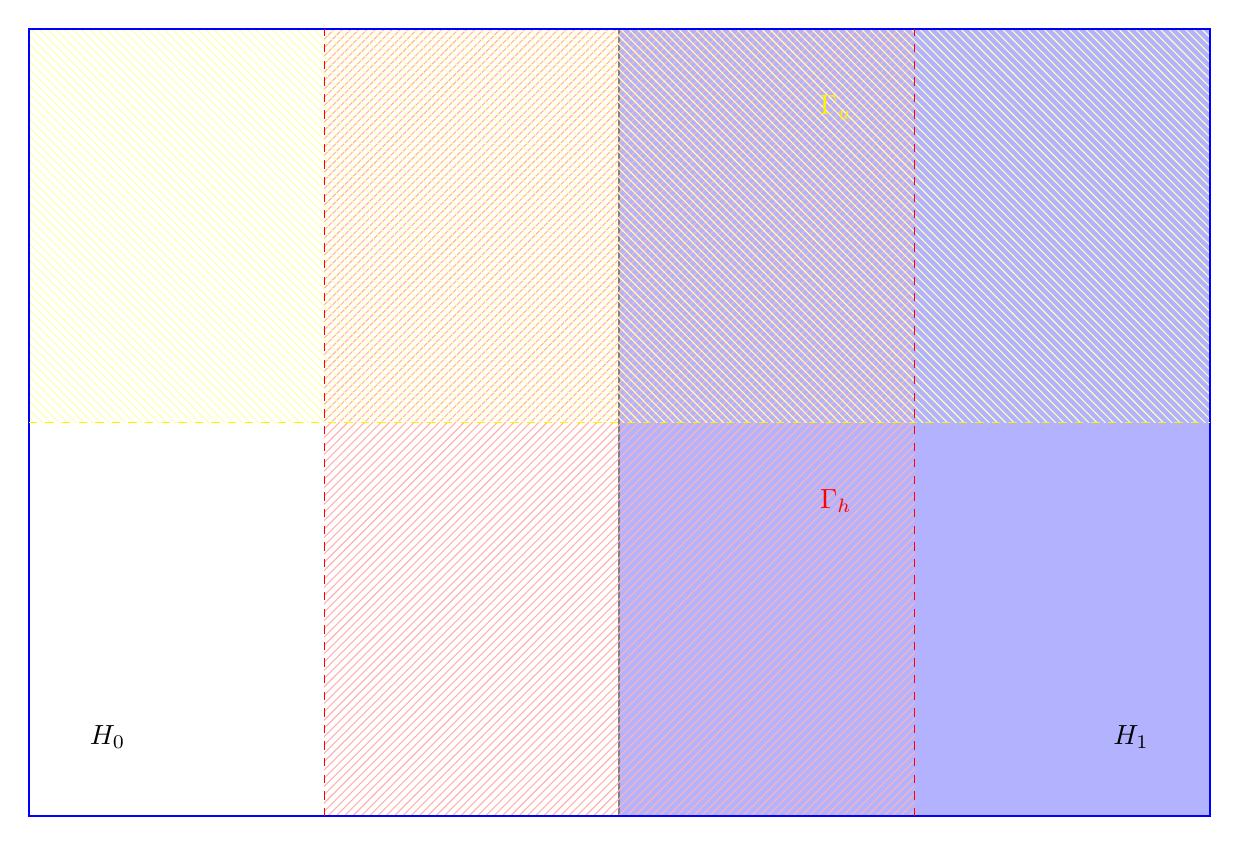
\begin{tikzpicture}
\fill[color=blue!30] (7.5,0) rectangle (15,10);
\draw[gray, thick] (7.5,0) -- (7.5,10);
\fill[pattern=north east lines, pattern color=red!30] (3.75,0) rectangle (11.25,10);
\fill[pattern=north west lines, pattern color=yellow!30] (0,5) rectangle (15,10);
\draw[blue, thick] (0,0) rectangle (15,10);
\draw[dashed, color=yellow] (0,5) -- (15,5);
\draw[dashed, color=red] (3.75,0) -- (3.75,10);
\draw[dashed, color=red] (11.25,0) -- (11.25,10);
\node[] at (1,1) {$H_0$};
\node[] at (14,1) {$H_1$};
\node[color=red] at (10.25,4) {$\Gamma_h$};
\node[color=yellow] at (10.25,9) {$\Gamma_u$};
\end{tikzpicture}
\caption{The cylinder $\Gamma_L$.}
\label{fig:setup}
\end{figure}

We also consider the plane $\Z^2$. In this setting, there are no edge states, and so the associated ``bulk" Hamiltonian $H_B$ is assumed to have a \textit{gapped} spectrum, in the sense that

\begin{assumption}
\[\emph{Spec}(H_B) = \mathcal{S}_{-} \cup \mathcal{S}_{+},\]
where $\inf\mathcal{S}_{+} - \sup \mathcal{S}_{-} \geq \gamma$ uniformly in $L$ and $\mu$ for some $\gamma > 0$. 
\label{ass:gap}
\end{assumption}

In the case of the cylinder, this effect does not necessarily occur due to the presence of the edge. 
We also assume that the Hamiltonian is \emph{locally charge-conserving}.

\begin{assumption}
$[\Phi(X),Q] = 0$, where $Q$ is the total charge in $\Gamma_L$.
\label{ass:charge}
\end{assumption}

Let $P_B$ be the ground state projection of $H_B$ (the system without an edge), and let $P$ be the ground state projection of $H$ (the system with an edge). We assume that states far from the edge are essentially bulk states, up to tails that vanish quickly in $L$.

\begin{assumption}
Define the \emph{edge region }

\[\Gamma_E = [L/2-k,L/2+k]\times [0,L] \cup [L-k,k]\times [0,L].\]

for some $k>0$. For any operator $A$ supported on $\Gamma_E^\mathsf{c}$,

\[\emph{Tr}(PA) = \emph{Tr}(P_BA) + \mathcal{O}(L^{-\infty}).\]

The $A$ on the right hand side is understood to be the extension by zeroes of $A$ to the plane $\Z^2$.
\label{ass:bulk}
\end{assumption}

The idea is that observables localized far away from the edge are not affected by the edge of the system. We similarly define the \emph{bulk region}

\[\Gamma_B = [3L/4-k, 3L/4+k] \times [0,L],\]

and the \emph{middle region}

\[\Gamma_m = [L/2,L]\cup[0,L] \setminus (\Gamma_E \cup \Gamma_B).\]

The three regions are depicted in figure \ref{fig:regions}.

\newpage
\begin{figure}[h!]
\centering
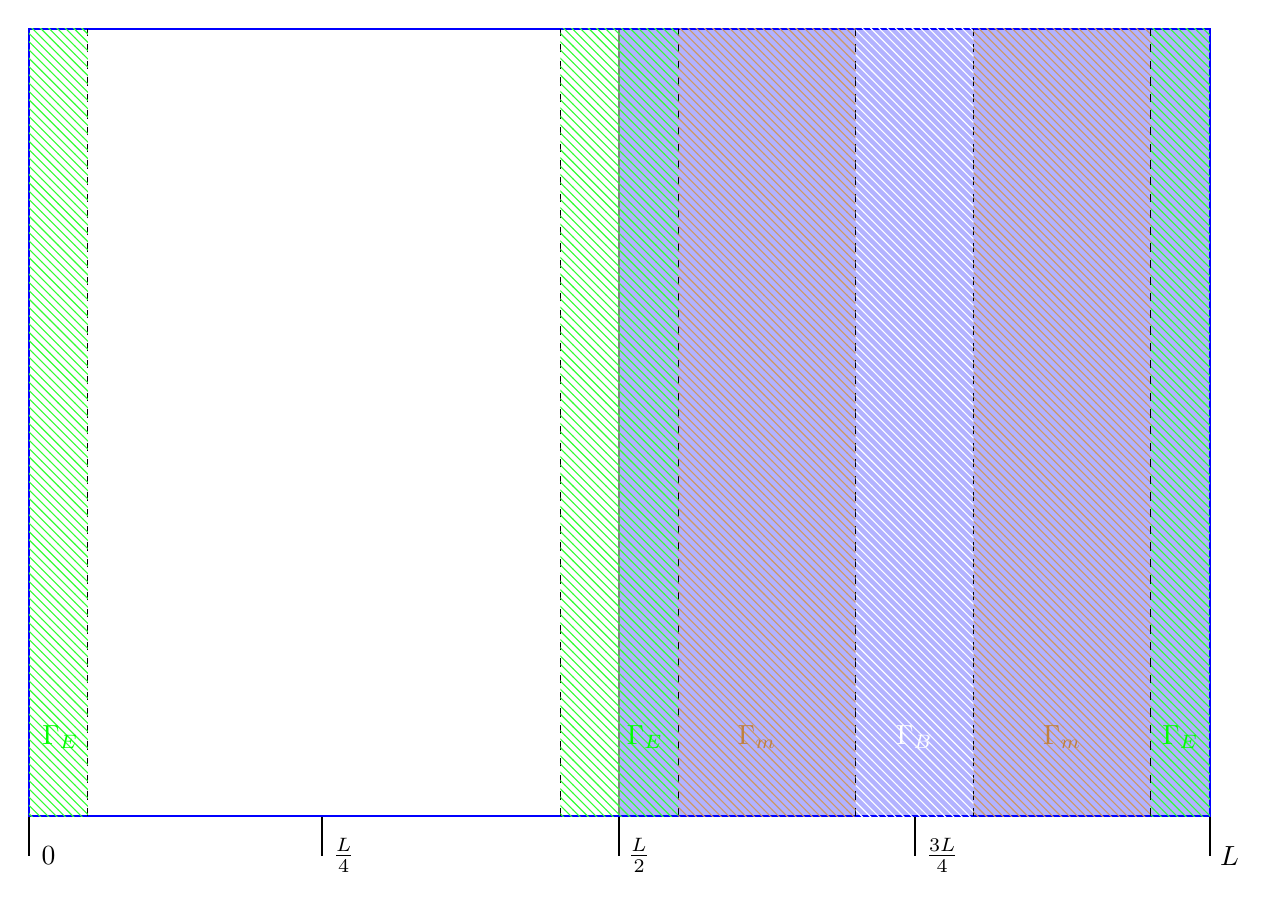
\begin{tikzpicture}
\fill[color=blue!30] (7.5,0) rectangle (15,10);
\draw[gray, thick] (7.5,0) -- (7.5,10);

\draw[black,thick] (0,-0.5) -- (0,0);
\node[] at (0.25,-0.5) {$0$};
\draw[black,thick] (3.725,-0.5) -- (3.725,0);
\node[] at (4,-0.5) {$\frac{L}{4}$};
\draw[black,thick] (7.5,-0.5) -- (7.5,0);
\node[] at (7.75,-0.5) {$\frac{L}{2}$};
\draw[black,thick] (11.25,-0.5) -- (11.25,0);
\node[] at (11.6,-0.5) {$\frac{3L}{4}$};
\draw[black,thick] (15,-0.5) -- (15,0);
\node[] at (15.25,-0.5) {$L$};

%\fill[pattern=north east lines, pattern color=red!30] (3.75,0) rectangle (11.25,10);
%\fill[pattern=north west lines, pattern color=yellow!30] (0,5) rectangle (15,10);
\draw[blue, thick] (0,0) rectangle (15,10);
%\draw[dashed, color=yellow] (0,5) -- (15,5);
%\draw[dashed, color=red] (3.75,0) -- (3.75,10);
%\draw[dashed, color=red] (11.25,0) -- (11.25,10);
%\node[] at (1,1) {$H_0$};
%\node[] at (14,1) {$H_1$};
%\node[color=red] at (10.25,4) {$\Gamma_h$};
%\node[color=yellow] at (10.25,9) {$\Gamma_u$};

\draw[dashed, color=black] (6.75,0) -- (6.75,10);
\draw[dashed, color=black] (8.25,0) -- (8.25,10);
\fill[pattern=north west lines, pattern color=green!80] (6.75,0) rectangle (8.25,10);
\node[color=green] at (7.825,1) {$\Gamma_E$};

%\draw[dashed, color=brown] (8.25,0) -- (8.25,10);
%\draw[dashed, color=brown] (10.5,0) -- (10.5,10);
\fill[pattern=north west lines, pattern color=brown!80] (8.25,0) rectangle (10.5,10);
\node[color=brown] at (9.25,1) {$\Gamma_m$};

\draw[dashed, color=black] (10.5,0) -- (10.5,10);
\draw[dashed, color=black] (12,0) -- (12,10);
\fill[pattern=north west lines, pattern color=white!80] (10.5,0) rectangle (12,10);
\node[color=white] at (11.25,1) {$\Gamma_B$};

%\draw[dashed, color=brown] (12,0) -- (12,10);
%\draw[dashed, color=brown] (14.25,0) -- (14.25,10);
\fill[pattern=north west lines, pattern color=brown!80] (12,0) rectangle (14.25,10);
\node[color=brown] at (13.125,1) {$\Gamma_m$};

\draw[dashed, color=black] (14.25,0) -- (14.25,10);
\fill[pattern=north west lines, pattern color=green!80] (14.25,0) rectangle (15,10);
\node[color=green] at (14.625,1) {$\Gamma_E$};

\draw[dashed, color=black] (0.75,0) -- (0.75,10);
\fill[pattern=north west lines, pattern color=green!80] (0,0) rectangle (0.75,10);
\node[color=green] at (0.4,1) {$\Gamma_E$};
\end{tikzpicture}
\caption{The regions $\Gamma_E$, $\Gamma_B$, and $\Gamma_m$.}
\label{fig:regions}
\end{figure}




\subsection{Equality of Bulk and Edge Currents}

\subsubsection{Cylinder Geometry}

Let $P_\mu$ be the (possibly degenerate) ground state projection of $H_\mu$. Let $Q_u = \sum_{x \in \Gamma_u} a_x^* a_x$ be the charge in the upper half of the cylinder $\Gamma_u = [0,L] \times [L/2,L]$ (the yellow region in Figure \ref{fig:setup}), and define current operator 

\[J = i[H_\mu,Q_u],\]

which measures the current across the fiducial line $y=L/2$. Charge conservation~\ref{ass:charge} implies that this current operator is supported along a strip of width $2R$ centred on the fiducial line $y=L/2$. Indeed, if we inspect a local interaction $\Phi(X)$ of range $R$ with support $(\Gamma_u)_R$, where $(X)_\alpha$ is the $\alpha$-shrinking of the set $X$, then clearly $\Phi(X)$ commutes with the charge outside $\Gamma_u$, so that $[\Phi(X), Q_u] = [\Phi(X), Q]$, which vanishes by the charge conservation assumption~\ref{ass:charge}. Similarly, if $\Phi(X)$ is supported in $((\Gamma_u)^\mathsf{c})_R$, then $[\Phi(X), Q_u] = [\Phi(X), Q] = 0$. It follows that for an interaction $\Phi(X)$ with range $R$ and arbitrary support, $[\Phi(X), Q_u]$ must be supported on a set which is contained in (or equal to) the strip $[L/2, L] \times [L/2-R, L/2+R]$. There $[H_\mu,Q_u]$ must be supported there as well, since $H_\mu$ is a sum of such local interactions. 

From this point, we drop the subscript $\mu$ wherever it is not needed for context.

% In the case of a unique ground state $\Omega$, the total change in charge in $\Gamma_h$ after threading one quantum of flux is given by the fundamental theorem of calculus,

%\[ \int_{t:\Phi = 0}^{t:\Phi=2\pi} i[H, Q_u] dt' = \langle \Omega, (U^* Q_h U - Q_h) \Omega \rangle\]

\begin{lemma}
The ground state expectation of the current $J$ is zero.
\label{lemma:J=0}
\end{lemma}

\begin{proof}
Assuming linearity and cyclicity of the trace hold, the proof is trivial, 

\[\begin{aligned}
\Tr(P J) = i\Tr(P [H,Q_u]) = i\Tr([P,H]Q_u) = 0.
\end{aligned}\]

In order for this calculation to hold, we need to prove that

\begin{enumerate}
\item $P H Q_u$ and $P Q_u H$ are separately trace-class to apply linearity of the trace, and 
\item $\norm{H}<\infty$ and $P Q_u \in \mathcal{J}_1$ to apply cyclicity of the trace. 
\end{enumerate}

The latter implies the former by the bound $\norm{AB}_1 \leq \norm{A}_1\norm{B}$.  To prove (2), fix a finite $L$. The Hamiltonian is bounded since it is a finite sum of at most $\mathcal{P}(\Gamma_L)$ local interactions $\Phi(X)$, each of which is uniformly bounded by assumption, along with the $\mu Q_h$ term. But the number operator for the entire space is bounded by $\norm{Q} \leq NL^2$, where $N$ is the uniform bound on the dimension of each Hilbert space. This shows that both $Q_u$ and $Q_h$ are bounded in operator norm. Finally, $\norm{P}_1\leq CL^2$ because the projection is finite-rank, since the dimension of each site is bounded. Therefore $P Q_u \in \mathcal{J}_1$.

%\[\begin{aligned}
%\norm{P_\mu H_\mu}_1 &= \norm{P_\mu\sum_{X\in \Gamma_L}\Phi(X) + P_\mu \mu Q_h}_1\\
%&\leq \sum_{X\in\Gamma_L} \norm{P_\mu \Phi(X)}_1 + \mu\norm{P_\mu Q_h}_1\\
%&\leq \norm{P_\mu}_1 \sum_{X\in\Gamma_L} \norm{\Phi(X)}+ \mu \norm{P_\mu}_1\norm{Q_h}\\
%\end{aligned}\]
\end{proof}

Next, we define a family of operators indexed by $\mu$ called \emph{Hastings operators},

\[K_\mu = \mathcal{I}_{\mu}(\dot{H}_\mu),\]

where 

\[\mathcal{I}_{\mu} (A) = \int_\R W(t) e^{itH_\mu} A e^{-itH_\mu}dt.\]

Here, $W:\R\to\R$ is a function satisfying (need to add). More explicitly, in our setting we see that 

\[K_\mu = \mathcal{I}_\mu(Q_h).\]

 %As a shorthand, we use the notation $\dot{A}_{\mu_0}= (\frac{d}{d\mu}A_\mu)|_{\mu=\mu_0}$. 

We present two important properties of the map $\mathcal{I}_\mu:\mathcal{U}_L\to\mathcal{U}_L$ in the following lemmas, and leave their proofs to the appendix (need to add). 

First, recall a definition from the non-interacting setting: an \emph{off-diagonal} operator is an operator $A$ such that $A = \overline{A} := P_\mu AP_\mu^\perp + P_\mu^\perp AP_\mu$, where $P_\mu^\perp = \mathbb{I} - P_\mu$ is the projection onto the excited states above the gap.

\begin{lemma}
\begin{enumerate}
\item For any off-diagonal operator $A=\overline{A}$, $\mathcal{I}_\mu(\cdot)$ and $[H_\mu, \cdot]$ act as inverses of each other, up to a factor of $i$:

\[\mathcal{I}_\mu\left([H_\mu, A]\right) = [H_\mu, \mathcal{I}_\mu(A)] = iA.\]

\item For any (not necessarily off-diagonal) operator $A$, 

\[[\mathcal{I}_\mu([H_\mu, A]),P_\mu] = i[A,P_\mu].\]
\end{enumerate}
\label{lemma:inverseofH}
\end{lemma}

%It is easy to verify that any operator $A$ behaves as an off-diagonal operator when taking a commutator with $P$, in the sense that

%\[[\overline{A}, P] = [A,P].\]

%Combining this fact with Lemma \ref{lemma:inverseofH}, it follows that for any (not necessarily off-diagonal) operator $A$, 

%\[[\mathcal{I}_\mu([H_\mu, A]),P_\mu] = i[A,P_\mu].\]

Another important property of the map $\mathcal{I}_\mu$ is that it preserves locality.

\begin{lemma}
$\mathcal{I}_\mu$ is local in the sense that for any $A \in \mathcal{U}_X$, 

\[\norm{\mathcal{I}(A)_{(X^r)^\mathsf{c}}} \leq \norm{A} |X| \mathcal{O}(r^{-\infty})\]

where $X^r = X \cup \{ x : d(x,X) \leq r\}$ is the $r$-fattening of $X$.
\label{lemma:local}
\end{lemma}

\begin{proposition}
The operator $K_\mu$ is the \emph{generator of parallel transport}, satisfying
\[\dot{P}_\mu = i[K_\mu,P_\mu]\]
for all $\mu$.
\label{prop:generatorparalleltransport}
\end{proposition}
\begin{proof}
First, we show that $\dot{P}$ is off-diagonal. Taking the derivative on both sides of $P^2=P$, we see that $\dot{P} P + P \dot{P} = \dot{P}$. Acting on the left and right with $P$ on both sides of this equation gives 

\[P\dot{P}P + P\dot{P}P = P\dot{P}P,\]

which implies that $P\dot{P}P = 0$. Thus 

\[\begin{aligned}
\overline{\partial_\mu P} &= P\dot{P}(1-P) + (1-P)\dot{P}P\\
&= P\dot{P} - P\dot{P}P + \dot{P}P - P\dot{P}P\\
&= P\dot{P} + \dot{P}P\\
&= \partial_\mu (P^2)\\
&= \partial_\mu P,
\end{aligned}\]

as claimed. By the product rule and the fact that $H$ and $P$ commute, 

\[ [\dot{H}, P] = -[H, \dot{P}]. \]

It therefore follows from Lemma~\ref{lemma:inverseofH} that 

\[\begin{aligned}
\dot{P} &= -i \mathcal{I}_\mu([H, \dot{P}]) = i\mathcal{I}([\dot{H}, P]) = i[\mathcal{I}(\dot{H}), P] = i[K, P].
\end{aligned}\]
\end{proof}

Increasing the electric potential by a small amount $d\mu Q_h$ and expanding to linear order, the change in ground state current is given by

\[\Tr(P_{\mu+d\mu}J) - \Tr(P_\mu J) = \kappa d\mu + \mathcal{O}(d\mu^2).\]

Dividing by $d\mu$ and taking a limit, we see that the linear response coefficient is given by

\[\sigma(\mu) = \Tr\left(\dot{P}_\mu J\right).\]

The \emph{Hall conductivity} of the system on a subset $V \subseteq \Gamma_L$ is defined to be $\sigma_V := \Tr\left(\dot{P} J_V\right)$, where $J_V$ is the restriction of $J$ to $V$. 

\begin{proposition}
The Hall conductivity is independent of the driving strength $\mu$.
\label{prop:independent}
\end{proposition}
\begin{proof}

%Since $\dot{H}_\mu=Q_h$, we see that $\dot{J} = 0$. Thus $\frac{d}{d\mu} \Tr(P_\mu J) = \sigma(\mu)$. 

For any $\mu_1$ and $\mu_2$,

%\[\begin{aligned}
%\sigma(\mu_1) - \sigma(\mu_2) &= \frac{d}{d\mu} \Tr\left( P_{\mu_1} i[H_{\mu_1}, Q_u] - P_{\mu_2}i[H_{\mu_2},Q_u]\right)\\
%&= i\frac{d}{d\mu} \Tr\left(\left([P_{\mu_1}, H_{\mu_1}] - [P_{\mu_2}, H_{\mu_2}]\right)Q_u\right)\\
%&= 0
%\end{aligned}\]
%^Doesn't work because otherwise \sigma=0 always.


\[\begin{aligned}
\sigma(\mu_1) - \sigma(\mu_2) &= \Tr\left( \dot{P}_{\mu_1} i[H_{\mu_1}, Q_u] - \dot{P}_{\mu_2}i[H_{\mu_2},Q_u]\right)\\
&= i\Tr\left(\left([\dot{P}_{\mu_1}, H_{\mu_1}] - [\dot{P}_{\mu_2}, H_{\mu_2}]\right)Q_u\right)\\
&= - i\Tr\left(\left([\dot{H}_{\mu_1}, P_{\mu_1}] - [\dot{H}_{\mu_2}, P_{\mu_2}]\right)Q_u\right)\\
&= i\Tr\left( [Q_h, P_{\mu_1} - P_{\mu_2}]Q_u \right)\\
&= i\Tr\left( [Q_u,Q_h]( P_{\mu_1} - P_{\mu_2})\right)\\
&= 0,
\end{aligned}\]
% Would need to bound \norm{\dot{P}}_1 to do this ^.

since $H$ and $P$ commute. Note that $\norm{\dot{P}}_1<\infty$ since we are working in a finite-dimensional space. The proof of Lemma \ref{lemma:J=0} provides the other necessary bounds to invoke linearity and cyclicity of the trace to shift the commutator in the second line and second-last line.
\end{proof}

This indicates that the Hall conductivity is independent of $\mu$ as one would expect physically. We simply write $\sigma=\sigma(\mu)$ from this point, in accordance with proposition \ref{prop:independent}. 

The following is the main result:

\begin{theorem}
Let $V \subseteq \Gamma_m$ be a set contained within the strip in between the edge region $\Gamma_E$ and the bulk region $\Gamma_B$ (see Figure \ref{fig:regions}), and define the distance

\[r = \emph{dist}(V, \Gamma_E \cup \Gamma_B)\]

from $V$ to the bulk and edge regions. The Hall conductivity in this regions vanishes in the sense that

\[\sigma_V = \mathcal{O}(r^{-\infty}) + \mathcal{O}(L^{-\infty}).\]

\end{theorem}

\begin{proof}
By Proposition~\ref{prop:generatorparalleltransport}, the bulk Hall conductivity can also be written by the formula 

\[\sigma_V^B = \Tr\left(i[K,P_B]J_V^B\right) = \Tr\left(i[\mathcal{I}(Q_h), P_B]J_V^B\right),\]

where $J_V^B = i[H_B, Q_u]|_V$ is the current in the region $V$ arising from the bulk Hamiltonian. From commutativity of $P_B$ and $H_B$ along with cyclicity of the trace, we compute

\[\begin{aligned}
\sigma_V^B &= \Tr\left(i\int_\R W(t) e^{itH_B} [Q_h,P_B] e^{-itH_B}dt J_V^B \right)\\
&= \int_\R W(t) \Tr\left(i[Q_h,P_B] e^{-itH_B}J_V^Be^{itH_B}\right)dt\\
&= -\int_\R W(t) \Tr\left(i[Q_h,P_B] e^{itH_B}J_V^Be^{-itH_B}\right)dt\\
&=- \Tr\left(i[Q_h,P_B]\mathcal{I}(J_V^B)\right),
\end{aligned}\]

since $W(t)$ is odd. By part (2) of Lemma \ref{lemma:inverseofH}, we have $i[Q_h,P_B] = [\mathcal{I}([H_B,Q_h]),P_B]$. Therefore

\[\begin{aligned}
\sigma_V^B &=-\Tr([\mathcal{I}([H_B,Q_h]), P_B]\mathcal{I}(J_V^B))\\
&= \Tr\left( P_B[\mathcal{I}([H_B,Q_h]), \mathcal{I}(J_V^B)]\right).
\end{aligned}\]

Now, $[H_B, Q_h]$ is a local operator supported on $\Gamma_B$, while $J_V^B$ is a local operator supported on $V \cap \Gamma_B = \varnothing$. Since $\mathcal{I}$ preserves locality up to tails, in the sense that $\norm{\mathcal{I}(A)_{(S^r)^\mathsf{c}}} \leq \norm{A} |S| \mathcal{O}(r^{-\infty})$ for any operator $A$ supported in $S$ (Lemma~\ref{lemma:local}), it follows that the commutator can be written

\[[\mathcal{I}([H_B,Q_h])|_{\Gamma_B} + \mathcal{O}(r^{-\infty}) A_1, \mathcal{I}(J_V^B)|_V + \mathcal{O}(r^{-\infty}) A_2] = C\mathcal{O}(r^{-\infty}),\]

for some operators $A_1$ and $A_2$ supported on $\Gamma_B^\mathsf{c}$ and $V^\mathsf{c}$, respectively. This fact applies to the bulk setting with $H_B$ and $P_B$. To extend this to the setting with an edge, it is enough to use Assumption~\ref{ass:bulk} to conclude the same result, except with equality up to $\mathcal{O}(L^{-\infty})$, i.e.

\[\sigma_V = \Tr\left(\dot{P}J_V\right) = \Tr\left(\dot{P}(J_V^B + \mathcal{O}(L^{-\infty}))\right) = \sigma_V^B + \mathcal{O}(L^{-\infty}) = \mathcal{O}(r^{-\infty}) + \mathcal{O}(L^{-\infty}).\]

\end{proof}


The intuitive picture from the previous result is that, in the bulk region, the Hall conductivity is essentially only nonzero along  the bulk strip $\Gamma_B$. Since the ground state expectation of the current is zero (by lemma~\ref{lemma:J=0}), it must be that there is an equal current flowing along the edge strip $\Gamma_E$, but in the opposite direction.

\subsubsection{Torus Geometry}

Our goal is to show the same result on the discrete torus $\mathbb{T}_L := \Z_L \times \Z_L$. We define the same regions $\Gamma_u$ and $\Gamma_h$, and the same current operator $J_u = i[H(\mu), Q_u]$. This time, however, Lemma~\ref{lemma:J=0} does not apply. Intuitively, it does not apply because electrons can now flow through both the bottom and the top of the region $\Gamma_u$, rather than just the bottom. Mathematically, the lemma fails because our definition of the current is slightly changed.

We use charge conservation and the fact that $H$ is finite range to split the current $J_u$ into two components, $J_u = i[H_-, Q_u] + i[H_+, Q_u] = J_- - J_+$, supported on strips of width $2R$ at $y=L/2$ and $y=L$, respectively. We then define the current operator to be $J=J_-$, which is the current on the lower strip. This is the mathematical reason that the proof in Lemma~\ref{lemma:J=0} fails on the torus; we have replaced $H$ by $H_-$, which may no longer commute with $P$. We instead proceed by a different approach. We will need a few auxiliary results first.

\begin{lemma}
$K_\pm$ is supported on $\partial_\pm$ up to tails.
\label{SupportOfK}
\end{lemma}
\begin{proof}

\end{proof}

\begin{proposition}
The operator $Q_h-K$ leaves the ground state space invariant, i.e. $[Q_h-K, P] = 0$.
\end{proposition}
\begin{proof}

\end{proof}


\begin{lemma}
Show that $\emph{Tr}(A,[Q_h,P])=0$ for all $A \in \mathcal{U}_{\text{edge}}$. This shows that $Q_h$ commutes with $P$ ``along the edge".
\label{lemma:[Q,P]=0}
\end{lemma}
\begin{proof}

Let $A \in \mathcal{U}_{\text{edge}}$. Since $H$ is charge conserving, we may choose a simultaneous eigenbasis of $H$ and the total charge $Q$, in which case $P$ and $Q$ commute. It follows that

\[\begin{aligned}
\Tr(A[Q_h, P]) = \Tr([A, Q_h] P) = \Tr([A, Q]P) = \Tr(A[Q,P]) = 0.
\end{aligned}\]



%\[\begin{aligned}
%\Tr(A [Q_h, P]) &= \Tr([A, Q_h]P)\\
%&= \Tr([P,A]Q_h)\\
%&= \sum_{x \in \Gamma_h} \Tr([P, A] c_x^*c_x)\\
%&= \sum_{x \in \Gamma_h} \Tr\left(\bigotimes_{y \in \text{supp}([P, A])} \left[P, A\right]_y c_x^*c_x\right)\\
%&= \sum_{x \in \Gamma_h} \Tr\left(\bigotimes_{y \in \text{supp}([P, A])} \left[P_y, A_y\right] c_x^*c_x\right)\\
%&= \sum_{x \in \Gamma_h} \prod_{y \in \text{supp}([P, A])} \Tr([P_y, A_y] c_x^*c_x)
%\end{aligned}\]

%The support of $[P, A]$ is the edge, so

%\[\begin{aligned}
%\Tr(A [Q_h, P]) &= \sum_{x \in \Gamma_h} \prod_{y \in \text{edge}} \Tr([P_y, A_y] c_x^*c_x)\\
%&= \sum_{x \in \Gamma_h} \prod_{y \in \text{edge}} \Tr((\mathbb{I}\otimes\ldots\otimes\mathbb{I}\otimes [P_y, A_y] \otimes\mathbb{I}\ldots\otimes\mathbb{I}) (\mathbb{I}\otimes \ldots \otimes\mathbb{I} \otimes c^*_xc_x \otimes \mathbb{I} \ldots\otimes\mathbb{I}))\\
%&= \sum_{x \in \Gamma_h} \prod_{y \in \text{edge}} \Tr(\mathbb{I}\otimes\ldots\otimes\mathbb{I}\otimes c_x^*c_x \otimes \mathbb{I} \otimes \ldots \otimes\mathbb{I} \otimes [P_y, A_y] \otimes\mathbb{I}\ldots)\\
%&= \sum_{x \in \Gamma_h} \prod_{y \in \text{edge}, \; y\neq x} \Tr(c_x^*c_x)\Tr([P_y, A_y]) + \sum_{x \in \Gamma_h \cap \text{edge}} \Tr(c_x^*c_x [P_x, A_x]).\\
%\end{aligned}\]

%Since the trace of any commutator is zero, the terms in the first sum vanish. Since $\Gamma_h \cap \text{edge} =\text{edge}$, we are left with

%\[\Tr(A[Q_h, P]) = \sum_{x \in \text{edge}} \Tr(c_x^*c_x[P_x, A_x]) = \sum_{x \in \text{edge}} \Tr(P_x[A_x, c_x^*c_x]).\]

%For any particular $x\in \text{edge}$, write $P_x = \sum_n |\psi_n \rangle \langle \psi_n |$, where the sum is over ground states, and 

%\[\langle \psi | [P_y, A_y]|\psi\rangle = \sum_n \langle \psi | \psi_n \rangle \langle\psi_n | A |\psi\rangle - \sum_n \langle \psi | A |\psi_n\rangle\langle\psi_n | \psi\rangle \]

%Want to show:

%\[\Tr([P_y, A_y]) = \ldots = 0\]

\end{proof}

Finally, we will prove that in the bulk system with Hamiltonian $H_B(\mu)$, the ground state expectation of the current vanishes faster than any power as $L \to \infty$.

\begin{lemma}
The ground state expectation of the current $J_B := i[(H_B)_-, Q_h]$ (of the system without an edge) is $\emph{Tr}(P_BJ_B)=\mathcal{O}(L^{-\infty})$.
\label{J=0Bulk}
\end{lemma}
\begin{proof}
First, $K = \mathcal{I}(i[H_B, Q])$ splits into $K = K_- - K_+$, with the support of $K_\pm$ contained in $\partial_\pm$ up to tails:

\[[K_\pm, A_X] = \mathcal{O}(p^{-\infty}),\]

for every $A_X \in \mathcal{U}_X$ such that $\norm{A_X}=1$, and where $p = \text{dist}(X, \partial_\pm)$ (need to add). Using the fact that $K_\pm$ is supported in $\partial_\pm$ up to tails (Lemma~\ref{SupportOfK}), we see that 

\[i[H_B, K_-] = i[(H_B)_-, K_-] + \mathcal{O}(L^{-\infty}),\]

and similarly $i[(H_B)_-, K_+] = \mathcal{O}(L^{-\infty})$. Putting these facts together, it follows that the current can be rewritten as 

\[\begin{aligned} 
J _B&= i[H_B, Q_h + K_- - K_- + K_+] + \mathcal{O}(L^{-\infty})\\
&= i[H_B, K_-] + i[(H_B)_-, Q_h - K_- + K_+)] + \mathcal{O}(L^{-\infty}).
\end{aligned}\]

From here, we use the fact that $H_B$ and $Q_h-K_-+K_+$ both commute with $P_B$ to write

\[P_BJ_BP_B = i[H_B, P_BK_-P_B] + i[P_B(H_B)_-P_B, Q_h - K_- + K_+)] + P_B\mathcal{O}(L^{-\infty})P_B.\]

Since the trace of any commutator is zero, 

\[\Tr(P_BJ_B) = \Tr(P_BJ_BP_B) = \mathcal{O}(L^{-\infty}).\]

\end{proof}

Using this, we can show a simple proof of the analogue of Lemma~\ref{lemma:J=0} on the torus, in the case of non-interacting systems.

\begin{proposition}
Let $H = \sum_{x \in \mathbb{T}} h_x$ be a non-interacting Hamiltonian, i.e. a sum of single site Hamiltonians $h_x$. The ground state expectation of the current $J=i[H_-, Q_h]$ (of the system with an edge) is $\emph{Tr}(PJ)=\mathcal{O}(L^{-\infty})$.
\label{prop:J=0Torus}
\end{proposition}

\begin{proof}

Since $H$ is a sum of single site Hamiltonians, we can split $H_-$ into the restrictions $H_- = (H_-)_\text{edge} + (H_-)_\text{bulk}$, with no fear of any terms which are in both the edge region and the bulk region. By Assumption~\ref{ass:bulk},

\[\begin{aligned}
\Tr(PJ) &= \Tr(Pi[H_-, Q_h])\\
&= i\Tr([H_-, Q_h]P)\\
&= i\Tr((H_-)_\text{edge} [Q_h, P]) + i \Tr((H_-)_\text{bulk} [Q_h, P])\\
&= i\Tr((H_-)_\text{edge} [Q_h, P]) + i \Tr((H_-)_\text{bulk} [Q_h, (P)_\text{bulk}])\\
&= i\Tr((H_-)_\text{edge} [Q_h, P]) + i \Tr((H_B)_-[Q_h, P_B]) + \mathcal{O}(L^{-\infty})\\
&= i\Tr((H_-)_\text{edge} [Q_h, P]) + \Tr(i[(H_B)_-, Q_h]P_B) + \mathcal{O}(L^{-\infty}).
\end{aligned}\]

By Lemma~\ref{lemma:[Q,P]=0}, the first term is zero. By Lemma~\ref{J=0Bulk}, the second term is $\mathcal{O}(L^{-\infty})$. 
\end{proof}









% Sections are a sub-unit
\section{A Section}
Here is a section with some text.  Equations look like this
$y=x$.\footnote{Here is a footnote.}

This is an example of a second paragraph in a section so you can
see how much it is indented by.

% Subsections follow
\subsection{This is a Subsection}
Here is an example of a citation: \cite{Forbes:2006ba}.  The actual
form of the citation is governed by the bibliographystyle.  These
citations are maintained in a BIBTeX file \texttt{sample.bib}.  You
could type these directly into the file.  For an example of the format
to use look at the file \texttt{ubcsample.bbl} after you compile this
file.\footnote{Here is another footnote.}

This is an example of a second paragraph in a subsection so you can
see how much it is indented by.

\subsubsection{This is a Subsubsection}
Here are some more citations \cite{LL3:1977,Peccei:1989,Turner:1999}.
If you use the \texttt{natbib} package with the \verb+sort&compress+
option, then the following citation will look the same as the first
citation in this section: \cite{Turner:1999,Peccei:1989,LL3:1977}.

This is an example of a second paragraph in a subsubsection so you can
see how much it is indented by.

\paragraph{This is a Paragraph}
Paragraphs and subparagraphs are the smallest units of text.  There is
no subsubsubsection etc.

\subparagraph{This is a Subparagraph}
This is the last level of organisation.  If you need more than this,
you should consider reorganizing your work\dots

\begin{equation}
  \mathrm{f}(x)=\int_{-\infty}^{\int_{-\infty}^x
    e^{-\frac{y^2}{2}}\mathrm{d}{y}}e^{-z^2}\mathrm{d}z
\end{equation}

In order to show you what a separate page would look like (i.e. without
a chapter heading) I must type some more text.  Thus I will babble a
bit and keep babbling for at least one more page\ldots  What you
should notice is that the chapter titles appear substantially lower
than the continuing text. Babble babble
babble babble babble babble babble babble babble babble babble babble
babble babble babble babble babble babble babble babble babble babble
babble babble babble babble babble babble babble babble babble babble
babble babble babble babble babble babble babble babble babble.

Babble babble babble babble babble babble babble babble babble babble
babble babble babble babble babble babble babble babble babble babble
babble babble babble babble babble babble babble babble babble babble
babble babble babble babble babble babble babble babble babble babble
babble babble babble babble babble babble babble babble babble babble
babble babble babble babble babble babble babble babble babble babble
babble babble babble babble babble babble babble babble babble babble
babble babble babble babble babble babble babble babble babble babble
babble babble babble babble babble babble babble babble babble babble
babble babble babble babble babble babble babble babble babble babble
babble babble babble babble babble babble babble babble babble babble
babble babble babble babble babble babble babble babble babble babble
babble babble babble babble.

\begin{table}[t]                 % optional [t, b or h];
  \begin{tabular}{|r||r@{.}l|}
    \hline
    Phoenix & \$960&35\\
    \hline
    Calgary & \$250&00\\
    \hline
  \end{tabular}
  \caption[Here is the caption for this wonderful table\ldots]{
    \label{tab:Table1}
    Here is the caption for this wonderful table. It has not been
    centered and the positioning has been specified to be at the top
    of the page.  Thus it appears above the babble rather than below
    where it is defined in the source file.}
\end{table}

% Force a new page: without this, the quote would appear on the
% previous page.
\newpage

\section{Quote}
Here is a quote:
\begin{quote}
  % It is centered
  \begin{center}
    This is a small poem,\\
    a little poem, a Haiku,\\
    to show you how to.\\
    ---Michael M$^{\rm c}$Neil Forbes.
  \end{center}
\end{quote}

This small poem shows several features:
\begin{itemize}
\item The use of the \verb|quote| and \verb|center| environments.
\item The \verb|\newpage| command has been used to force a page
  break.  (Sections do not usually start on a new page.)
\item The pagestyle has been set to suppress the headers using the
  command \verb|\thispagestyle{plain}|.  Note that using
  \verb|\pagestyle{plain}| would have affected all of the subsequent
  pages.
\end{itemize}
\section{Programs}
Here we give an example of a new float as defined using the
\texttt{float} package.  In the preamble we have used the commands
\begin{verbatim}
\floatstyle{ruled}
\newfloat{Program}{htbp}{lop}[chapter]
\end{verbatim}
This creates a ``Program'' environment that may be used for program
fragments.  A sample \texttt{python} program is shown in
Program~\ref{prog:fib}.  (Note that Python places a fairly restrictive
limit on recursion so trying to call this with a large $n$ before
building up the cache is likely to fail unless you increase the
recursion depth.)
\begin{Program}
  \caption{\label{prog:fib} Python program that computes the $n^{\rm
      th}$ Fibonacci number using memoization.}
\begin{verbatim}
def fib(n,_cache={}):
    if n < 2:
        return 1
    if n in _cache:
        return _cache[n]
    else:
        result = fib(n-1)+fib(n-2)
        _cache[n] = result
        return result
\end{verbatim}
\end{Program}
Instead of using a \texttt{verbatim} environment for your program
chunks, you might like to \texttt{include} them within an
\texttt{alltt} envrironment by including the \verb|\usepackage{alltt}|
package (see page 187 of the \LaTeX{} book).  Another useful package
is the \verb|\usepackage{listings}| which can pretty-print many
different types of source code.

% Force a new page
\newpage

%% Here we provide a short optional argument to \chapter[]{}.  This
%% optional argument will appear in the table of contents.  For long
%% titles, one should use this to give a single-line entry to the
%% table of contents.
\chapter[Another Chapter\ldots]{Another Chapter with a Very Long
  Chapter-name that will Probably Cause Problems}
\label{cha:apple_ref}

This chapter name is very long and does not display properly in the
running headers or in the table of contents.  To deal with this, we
provide a shorter version of the title as the optional argument to the
\verb|\chapter[]{}| command.

For example, this chapter's title and associated table of contents heading and
running header was created with\\
\verb|\chapter[Another Chapter\ldots]{Another Chapter with a Very Long|\\
\verb|Chapter-name that will Probably Cause Problems}|.

Note that, according to the thesis regulations, the heading included
in the table of contents must be a truncation of the actual heading.

This Chapter was used as a demonstration in the Preface for how to
attribute contribution from collaborators.  If there are any such
contributions, details must be included in the Preface.  If you wish,
you may additionally use a footnote such as this.\footnote{This
  chapter is based on work conducted in UBC's Maple Syrup Laboratory
  by Dr. A. Apple, Professor B. Boat, and C. Cat.}

\section{Another Section}
Another bunch of text to demonstrate what this file does.
You might want a list for example:\footnote{Here is a footnote in a
  different chapter.  Footnotes should come after punctuation.}
\begin{itemize}
\item An item in a list.
\item Another item in a list.
\end{itemize}

\section*{An Unnumbered Section That is Not Included in the Table of
  Contents}
\begin{figure}[ht]
  \begin{center}
%% psfrag: comment the following line if not using the psfrag package
    \psfrag{pie makes me happy!}{$\pi$ makes me happy!}
%% includegraphics: comment the following if not using the graphicx package
    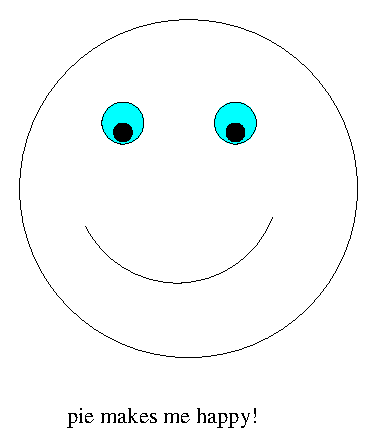
\includegraphics[width=0.4\textwidth]{fig}
    \caption[Happy Face: figure example.]{\label{fig:happy} This is a figure of
      a happy face with a \texttt{psfrag} replacement.  The original figure
      (drawn in xfig and exported to a .eps file) has the text ``pie makes me
      happy!''.  The \texttt{psfrag} package replaces this with ``$\pi$ makes me
      happy!''.  Note: the Makefile compiles the sample using pdf\LaTeX\ which
      cannot use \texttt{psfrag} directly.  For some options that work with
      pdf\LaTeX, please see this discussion:
      \url{http://tex.stackexchange.com/questions/11839}.  For the caption, we
      have used the optional argument for the caption command so that only a
      short version of this caption occurs in the list of figures.}
  \end{center}
\end{figure}
\afterpage{\clearpage}
Here is an example of a figure environment.
Perhaps I should say that the example of a figure can be seen in
Figure~\ref{fig:happy}.  Figure placement can be tricky with \LaTeX\
because figures and tables are treated as ``floats'': text can flow
around them, but if there is not enough space, they will appear later.
To prevent figures from going too far, the
\verb|\afterpage{\clearpage}| command can be used.  This makes sure
that the figure are typeset at the end of the page (possibly appear on
their own on the following pages) and before any subsequent text.

The \verb|\clearpage| forces a page break so that the figure can be
placed, but without the the \verb|\afterpage{}| command, the page
would be broken too early (at the \verb|\clearpage| statement).  The
\verb|\afterpage{}| command tells \LaTeX{} to issue the command after
the present page has been rendered.

\section{Tables}
We have already included one table:~\ref{tab:Table1}.  Another table
is plopped right here.
\begin{table}[ht]
  \begin{center}
    \begin{tabular}{|l||l|l||l|l|}
      \hline
      &\multicolumn{2}{l|}{Singular}&\multicolumn{2}{l|}{Plural}\\
      \cline{2-5}
       &English&\textbf{Gaeilge}&English&\textbf{Gaeilge}\\
      \hline\hline
      1st Person&at me&\textbf{agam}&at us&\textbf{againn}\\
      2nd Person&at you&\textbf{agat}&at you&\textbf{agaibh}\\
      3rd Person&at him&\textbf{aige}&at them&\textbf{acu}\\
       &at her&\textbf{aici}& & \\
      \hline
    \end{tabular}
    \caption{
      \label{tab:Table2}
      Another table.}
  \end{center}
\end{table}
Well, actually, as with Figures, tables do not
necessarily appear right ``here'' because tables are also ``floats''.
\LaTeX{} puts them where it can.  Because of this, one should refer to
floats by their labels rather than by their location.  This example is
demonstrated by Table~\ref{tab:Table2}.  This one is pretty close,
however.  (Note: you should generally not put tables or figures in the
middle of a paragraph.  This example is for demonstration purposes
only.)

Another useful package is \verb|\usepackage{longtable}| which provides
the \texttt{longtable} environment.  This is nice because it allows
tables to span multiple pages.  Table~\ref{tab:longtable} has been
formatted this way.
\begin{center}
  \begin{longtable}{|l|l|l|}
    \caption{\label{tab:longtable}Feasible triples for
      highly variable Grid}\\

    \hline \multicolumn{1}{|c|}{\textbf{Time (s)}} &
    \multicolumn{1}{c|}{\textbf{Triple chosen}} &
    \multicolumn{1}{c|}{\textbf{Other feasible triples}} \\ \hline
    \endfirsthead

    \multicolumn{3}{c}%
    {{\bfseries \tablename\ \thetable{} -- continued from previous page}} \\
    \hline \multicolumn{1}{|c|}{\textbf{Time (s)}} &
    \multicolumn{1}{c|}{\textbf{Triple chosen}} &
    \multicolumn{1}{c|}{\textbf{Other feasible triples}} \\ \hline
    \endhead

    \hline \multicolumn{3}{|r|}{{Continued on next page}} \\ \hline
    \endfoot

    \hline \hline
    \endlastfoot

    0 & (1, 11, 13725) & (1, 12, 10980), (1, 13, 8235), (2, 2, 0), (3, 1, 0) \\
    274 & (1, 12, 10980) & (1, 13, 8235), (2, 2, 0), (2, 3, 0), (3, 1, 0) \\
    5490 & (1, 12, 13725) & (2, 2, 2745), (2, 3, 0), (3, 1, 0) \\
    8235 & (1, 12, 16470) & (1, 13, 13725), (2, 2, 2745), (2, 3, 0), (3, 1, 0) \\
    10980 & (1, 12, 16470) & (1, 13, 13725), (2, 2, 2745), (2, 3, 0), (3, 1, 0) \\
    13725 & (1, 12, 16470) & (1, 13, 13725), (2, 2, 2745), (2, 3, 0), (3, 1, 0) \\
    16470 & (1, 13, 16470) & (2, 2, 2745), (2, 3, 0), (3, 1, 0) \\
    19215 & (1, 12, 16470) & (1, 13, 13725), (2, 2, 2745), (2, 3, 0), (3, 1, 0) \\
    21960 & (1, 12, 16470) & (1, 13, 13725), (2, 2, 2745), (2, 3, 0), (3, 1, 0) \\
    24705 & (1, 12, 16470) & (1, 13, 13725), (2, 2, 2745), (2, 3, 0), (3, 1, 0) \\
    27450 & (1, 12, 16470) & (1, 13, 13725), (2, 2, 2745), (2, 3, 0), (3, 1, 0) \\
    30195 & (2, 2, 2745) & (2, 3, 0), (3, 1, 0) \\
    32940 & (1, 13, 16470) & (2, 2, 2745), (2, 3, 0), (3, 1, 0) \\
    35685 & (1, 13, 13725) & (2, 2, 2745), (2, 3, 0), (3, 1, 0) \\
    38430 & (1, 13, 10980) & (2, 2, 2745), (2, 3, 0), (3, 1, 0) \\
    41175 & (1, 12, 13725) & (1, 13, 10980), (2, 2, 2745), (2, 3, 0), (3, 1, 0) \\
    43920 & (1, 13, 10980) & (2, 2, 2745), (2, 3, 0), (3, 1, 0) \\
    46665 & (2, 2, 2745) & (2, 3, 0), (3, 1, 0) \\
    49410 & (2, 2, 2745) & (2, 3, 0), (3, 1, 0) \\
    52155 & (1, 12, 16470) & (1, 13, 13725), (2, 2, 2745), (2, 3, 0), (3, 1, 0) \\
    54900 & (1, 13, 13725) & (2, 2, 2745), (2, 3, 0), (3, 1, 0) \\
    57645 & (1, 13, 13725) & (2, 2, 2745), (2, 3, 0), (3, 1, 0) \\
    60390 & (1, 12, 13725) & (2, 2, 2745), (2, 3, 0), (3, 1, 0) \\
    63135 & (1, 13, 16470) & (2, 2, 2745), (2, 3, 0), (3, 1, 0) \\
    65880 & (1, 13, 16470) & (2, 2, 2745), (2, 3, 0), (3, 1, 0) \\
    68625 & (2, 2, 2745) & (2, 3, 0), (3, 1, 0) \\
    71370 & (1, 13, 13725) & (2, 2, 2745), (2, 3, 0), (3, 1, 0) \\
    74115 & (1, 12, 13725) & (2, 2, 2745), (2, 3, 0), (3, 1, 0) \\
    76860 & (1, 13, 13725) & (2, 2, 2745), (2, 3, 0), (3, 1, 0) \\
    79605 & (1, 13, 13725) & (2, 2, 2745), (2, 3, 0), (3, 1, 0) \\
    82350 & (1, 12, 13725) & (2, 2, 2745), (2, 3, 0), (3, 1, 0) \\
    85095 & (1, 12, 13725) & (1, 13, 10980), (2, 2, 2745), (2, 3, 0), (3, 1, 0) \\
    87840 & (1, 13, 16470) & (2, 2, 2745), (2, 3, 0), (3, 1, 0) \\
    90585 & (1, 13, 16470) & (2, 2, 2745), (2, 3, 0), (3, 1, 0) \\
    93330 & (1, 13, 13725) & (2, 2, 2745), (2, 3, 0), (3, 1, 0) \\
    96075 & (1, 13, 16470) & (2, 2, 2745), (2, 3, 0), (3, 1, 0) \\
    98820 & (1, 13, 16470) & (2, 2, 2745), (2, 3, 0), (3, 1, 0) \\
    101565 & (1, 13, 13725) & (2, 2, 2745), (2, 3, 0), (3, 1, 0) \\
    104310 & (1, 13, 16470) & (2, 2, 2745), (2, 3, 0), (3, 1, 0) \\
    107055 & (1, 13, 13725) & (2, 2, 2745), (2, 3, 0), (3, 1, 0) \\
    109800 & (1, 13, 13725) & (2, 2, 2745), (2, 3, 0), (3, 1, 0) \\
    112545 & (1, 12, 16470) & (1, 13, 13725), (2, 2, 2745), (2, 3, 0), (3, 1, 0) \\
    115290 & (1, 13, 16470) & (2, 2, 2745), (2, 3, 0), (3, 1, 0) \\
    118035 & (1, 13, 13725) & (2, 2, 2745), (2, 3, 0), (3, 1, 0) \\
    120780 & (1, 13, 16470) & (2, 2, 2745), (2, 3, 0), (3, 1, 0) \\
    123525 & (1, 13, 13725) & (2, 2, 2745), (2, 3, 0), (3, 1, 0) \\
    126270 & (1, 12, 16470) & (1, 13, 13725), (2, 2, 2745), (2, 3, 0), (3, 1, 0) \\
    129015 & (2, 2, 2745) & (2, 3, 0), (3, 1, 0) \\
    131760 & (2, 2, 2745) & (2, 3, 0), (3, 1, 0) \\
    134505 & (1, 13, 16470) & (2, 2, 2745), (2, 3, 0), (3, 1, 0) \\
    137250 & (1, 13, 13725) & (2, 2, 2745), (2, 3, 0), (3, 1, 0) \\
    139995 & (2, 2, 2745) & (2, 3, 0), (3, 1, 0) \\
    142740 & (2, 2, 2745) & (2, 3, 0), (3, 1, 0) \\
    145485 & (1, 12, 16470) & (1, 13, 13725), (2, 2, 2745), (2, 3, 0), (3, 1, 0) \\
    148230 & (2, 2, 2745) & (2, 3, 0), (3, 1, 0) \\
    150975 & (1, 13, 16470) & (2, 2, 2745), (2, 3, 0), (3, 1, 0) \\
    153720 & (1, 12, 13725) & (2, 2, 2745), (2, 3, 0), (3, 1, 0) \\
    156465 & (1, 13, 13725) & (2, 2, 2745), (2, 3, 0), (3, 1, 0) \\
    159210 & (1, 13, 13725) & (2, 2, 2745), (2, 3, 0), (3, 1, 0) \\
    161955 & (1, 13, 16470) & (2, 2, 2745), (2, 3, 0), (3, 1, 0) \\
    164700 & (1, 13, 13725) & (2, 2, 2745), (2, 3, 0), (3, 1, 0) \\
\end{longtable}
\end{center}

\subsection*{An Unnumbered Subsection}
Note that if you use subsections or further divisions under an
unnumbered section, then you should make them unnumbered as well
otherwise you will end up with zeros in the section numbering.

\chapter{Landscape Mode}
The landscape mode allows you to rotate a page through 90 degrees.  It
is generally not a good idea to make the chapter heading landscape,
but it can be useful for long tables etc.

\begin{landscape}
  This text should appear rotated, allowing for formatting of very
  wide tables etc.  Note that this might only work after you convert
  the \texttt{dvi} file to a postscript (\texttt{ps}) or \texttt{pdf}
  file using \texttt{dvips} or \texttt{dvipdf} etc.  This feature is
  provided by the \verb|lscape| and the \verb|pdflscape| packages.
  The latter is preferred if it works as it also rotates the pages in
  the pdf file for easier viewing.
\end{landscape}

%% This file is setup to use a bibtex file sample.bib and uses the
%% plain style.  Other styles may be used depending on the conventions
%% of your field of study.
%%
%%% Note: the bibliography must come before the appendices.
\bibliographystyle{plain}
\bibliography{sample}

%% Use this to reset the appendix counter.  Note that the FoGS
%% requires that the word ``Appendices'' appear in the table of
%% contents either before each appendix lable or as a division
%% denoting the start of the appendices.  We take the latter option
%% here.  This is ensured by making the \texttt{appendicestoc} option
%% a default option to the UBC thesis class.

%%% If you only have one appendix, please uncomment the following line.
% \renewcommand{\appendicesname}{Appendix}
















%\newpage
%\appendix

\appendix
\chapter{General Functional Analysis}

\begin{lemma}
Let $A$ be a bounded linear operator on a Hilbert space $\mathcal{H}$. Suppose $A_n \xrightarrow{\enskip s \enskip} A$ on a dense subspace $\mathcal{D}\subset \mathcal{H}$. If $A_n$ are bounded uniformly in $n$, then $A_n \xrightarrow{\enskip s \enskip} A$ on all of $\mathcal{H}$.
\label{lemma:densesubspace}
\end{lemma}
\begin{proof}
Let $\psi_n \in\mathcal{D}$ be a sequence converging in norm to $\psi\in\mathcal{H}$. The result follows from a standard $\frac{\eps}{3}$ argument. Let $C$ be a bound for both $\sup_n \norm{A_n}$ and $\norm{A}$. Then 

\[\begin{aligned}
\norm{A_n\psi-A\psi} &\leq \norm{A_n(\psi-\psi_m)} + \norm{(A_n-A)\psi_m} + \norm{A(\psi-\psi_m)}\\
&\leq C\norm{(\psi-\psi_m)} + \norm{(A_n-A)\psi_m} + C\norm{\psi-\psi_m}.
\end{aligned}\]

There exists an $M$ such that the first and third terms are less than $\frac{\epsilon}{3}$ for all $m>M$. For the middle term, observe that for each $m$, there exists by hypothesis an $N_m$ such that $\norm{(A_n-A)\psi_m} < \frac{\epsilon}{3}$ for all $n>N_m$. Thus, by picking some $m>M$ and fixing a suitably large $n$, the inequality above is less than $\eps$.
\end{proof}




\section{Spectral Measures and Projection-Values Measures}\label{sec:pvm}

\emph{Projection-valued measures} are maps $P:\mathcal{M}\to\mathcal{B}(\mathcal{H})$ from measurable subsets of $\R$ to the space of bounded linear operators on $\mathcal{H}$ satisfying the usual properties of both projections and measures.

\begin{enumerate}
\item $P(M)=P(M)^*=P(M)^2$ is an orthogonal projection for all $M\in\mathcal{M}$. Note that this implies that $P(M)$ is a positive operator.
\item $P(\varnothing)=0$ and $P(\R)=\One_\mathcal{H}$.
\item If $\{M_i\}_{i\in\N}$ are pairwise disjoint, then $\sum_{i=1}^n P(M_i) \xrightarrow{\enskip s \enskip}P(\cup_{i\in\N} M_i)$ as $n\to\infty$ ($\sigma$-additivity).
\item $P(M_1\cap M_2) = P(M_1)P(M_2)$ for any $M_1,M_2\in\mathcal{M}$.
\end{enumerate}

The heuristic motivation is that $P(M)$ projects onto the subspace of $\mathcal{H}$ spanned by states whose energies lie in $M$. Using these operator-valued measures, one can construct an operator-valued integral with respect to $P$ in the usual fashion (beginning on nonnegative simple functions, extending to nonnegative measurable functions, and finally to real-valued measurable functions). 

\begin{theorem}[Spectral Theorem for Projection-Valued Measures]
There exists a one-to-one correspondence between self adjoint operators $H$ and projection-valued measures $P$ given by the formula
\[H = \int_\R \lambda dP_\lambda,\]
where $P_\lambda := P((-\infty,\lambda])$. Moreover, if $g:\R\to\R$ is any bounded Borel function, then $g(H)$ defined via the Borel function calculus coincides with the formula
\[g(H) = \int_\R g(\lambda) dP_\lambda,\]
and $g(H) = g(H)^*$.
\label{thm:spectraltheorem}
\end{theorem}

We remark that it follows from the second part of this theorem that if $\One_{M}$ denotes the characteristic function of a Borel set $M\subseteq \R$, then 

\[\One_M(H) = \int_M dP_\lambda = P(M).\]

We also note that $\text{Spec}(H) = \text{supp}(P)$.

\begin{lemma}
Let $A$ be a trace-class operator. If $\tr_X(A)$ denotes the partial trace of $A$ over the set $X$, then
\[\int_\mathcal{G} UAU^*d\mu(U) = \frac{1}{\emph{dim}(X)}\tr_X(A)\otimes \One,\]
where $\mu$ is the Haar measure on the group $\mathcal{G}$ of unitary operators supported in $X$.
\end{lemma}
\begin{proof}
Since the Haar measure is unique up to scalar multiple, we take without loss of generality $\mu(\mathcal{G})=1$. By left and right invariance of the Haar measure, 
\[\int_\mathcal{G} UAU^* d\mu(U) = \int_\mathcal{G} Ad\mu(U) = A.\]
The only operator invariant under all basis transformations is the identity, so
\[\alpha \One=\int_\mathcal{G} UAU^*d\mu(U)\]
for some scalar $\alpha$. Taking the partial trace over $X$, 
\[\alpha \text{dim}(X)\One_{X^\mathsf{c}} = \int_\mathcal{G} \tr_X(UAU^*)d\mu(U) = \int_\mathcal{G} \tr_X(A)d\mu = \tr_X(A).\]
Tensoring with $\One_X$ gives 
\[\alpha \One = \frac{1}{\text{dim}(X)} \tr_X(A) \otimes \One.\]
Need to add.
\end{proof}





\section{Greens' Functions and the Combes-Thomas Bound}

The short-range assumption \ref{ass:shortrange} is vital for the following non-trivial estimate, the proof of which is omitted.

\begin{theorem}[Combes-Thomas Bound]
Let $H$ be a self-adjoint operator on $\ell^2(\Z^2)$ satisfying

\[S_\alpha := \sup_x \sum_y |H(x,y)|(e^{\alpha|x-y|}-1) < \infty\]

for some $\alpha>0$. Suppose $z$ lies outside the spectrum of $H$, and let $d_z := \emph{dist}(z,\emph{Spec}(H))$.  Then the Greens function of $H$ is exponentially bounded, 

\[|G(x,y;z)| \leq \frac{2}{d_z}e^{-\xi_\alpha|x-y|},\]

where $\xi := \frac{\alpha d_z}{2 S_\alpha}$.
\label{thm:combesthomas}
\end{theorem}

This theorem gives the crucial decay properties of the spectral projectors.

\begin{lemma}
Let $H$ be a self-adjoint operator satisying \ref{ass:shortrange} and with bounded spectrum. Let $S \subseteq \emph{Spec}(H)$, and let $P_S$ be the associated spectral projection. Then there exists some $\eps,\nu>0$ such that the matrix elements of $P_S$ satisfy

\[\sum_{x,y \in \Z^2} |P_S(x,y)| e^{-\eps |x|} e^{\nu |x-y|} < \infty.\]
\label{lemma:projectionmatrixelementsdecay}
\end{lemma}
\begin{proof}
We use the fact that the spectral projection is given by the Riesz integral formula

\[P_S = \frac{1}{2\pi i} \oint_\gamma R(z)dz,\]

where $R(z)$ is the resolvent of $H$ and $\gamma$ is any smooth closed curve containing $S$. Since the resolvent is the Greens function of $H$, it satisfies the Combes-Thomas bound \ref{thm:combesthomas}. Since the spectrum of $H$ is bounded, it may be enclosed in a curve of finite length, from which we determine that

\[|P_S(x,y)| \leq Ce^{-\xi_\alpha|x-y|},\]

since $\inf_{z \in \gamma} d_z = \inf_{z\in\gamma} \text{dist}(z,\text{Spec}(H)) > 0$. Hence

\[\sum_{x,y \in \Z^2} |P_S(x,y)| e^{-\eps |x|} e^{\nu |x-y|} < \infty\]

holds for $\nu = \xi_\alpha$ and for any $\eps>0$, since $e^{-\eps|x|} = e^{-\eps|x_1|}e^{-\eps|x_2|}$ is summable on $\Z^2$ by Lemma \ref{lemma:exptraceclass}.

\end{proof}

This statement about decay of the matrix elements can be turned into a statement about the norm of the operator. Let $\text{Lip}^1$ be the set of all Lipschtiz functions whose Lipschitz constant is not greater than 1, that is the set of functions $\ell$ satisfying 

\[|\ell(x)-\ell(y)| \leq |x-y|\]

for all $x,y \in \Z^2$.

\begin{lemma}
Let $P_S$ be the spectral projection onto $S \subseteq \emph{Spec}(H)$. For all $\eps>0$,
\[\sup_{\ell \in \emph{Lip}^1} \norm{e^{\nu \ell(x)} e^{-\eps|x|} P_S e^{-\nu\ell(x)}} < \infty,\]
where $\nu$ is the same as in \ref{lemma:projectionmatrixelementsdecay}.
\label{lemma:projectionoperatordecay}
\end{lemma}
\begin{proof}
The matrix elements of the operator are $P_S(x,y) e^{\nu (\ell(x)-\ell(y))}e^{-\eps|x|}$. By Holmgren's bound, the operator's norm is therefore bounded by 

\[\max\{\sup_x \sum_y |P_S(x,y)| e^{\nu (\ell(x)-\ell(y))}e^{-\eps|x|}, \; \sup_y \sum_x|P_S(x,y)| e^{\nu (\ell(x)-\ell(y))}e^{-\eps|x|}\}.\]

Replacing the supremum with a sum yields the bound

\[\norm{P_S(x,y) e^{\nu (\ell(x)-\ell(y))}e^{-\eps|x|}} \leq \sum_{x,y} |P_S(x,y)| e^{\nu |\ell(x)-\ell(y)|}e^{-\eps|x|},\]

and taking a supremum over $\ell \in \text{Lip}^1$ completes the proof by Lemma \ref{lemma:projectionmatrixelementsdecay}.
\end{proof}






\chapter{Properties of $\mathcal{I}_\mu$}

\begin{proof}
(Of Lemma~\ref{lemma:inverseofH}). Let $\widehat{W}(\xi) = \frac{1}{\sqrt{2\pi}}\int_\R W(t) e^{-2\pi i t \xi} dt$ be the Fourier transform of $W$. One can show that for $|\xi|\geq \gamma$, $\widehat{W}(\xi) = \frac{1}{\sqrt{2\pi}i \xi}$ (need to add). Let $A$ be an observable. First, we show that $\mathcal{I}([H,PAP^\perp]) = iPAP^\perp$. 

Decomposing 

\[\begin{aligned}
e^{itH}P &= \sum_{j=0}^\infty \frac{(itH)^j}{j!} P \\
&= \sum_{j =0}^\infty \frac{(it)^j}{j!} \left(\sum_n E_n^j P_n\right)P \\
&= \sum_{j=0}^\infty \frac{(it)^j}{j!} \sum_{n : E_n=0} E_n^j P_n \\
&= \sum_{n : E_n=0} e^{itE_n}P_n,
\end{aligned}\]

and similarly 

\[P^\perp e^{-itH}= \sum_{m:E_m \geq \gamma}P_m e^{-itE_m},\]

we see that

\[\begin{aligned}
\mathcal{I}([H,PAP^\perp]) &= \mathcal{I}(P[H,A]P^\perp) \\
&= \int_\R W(t)e^{itH}P[H,A]P^\perp e^{-itH}dt \\
&= \int_\R W(t) \sum_{n : E_n=0} e^{itE_n}P_n [H,A] \sum_{m:E_m \geq \gamma} P_m e^{-itE_m} dt\\
&= \sum_{n : E_n=0} \sum_{m:E_m \geq \gamma} \int_\R W(t) e^{itE_n} P_n A (E_n-E_m) P_m e^{-itE_m}dt\\
&= \sum_{n : E_n=0} \sum_{m:E_m \geq \gamma} P_n A P_m (E_n-E_m) \int_\R W(t) e^{-it(E_m - E_n)} dt\\
&= \sum_{n : E_n=0} \sum_{m:E_m \geq \gamma} P_n A P_m (E_n-E_m) \sqrt{2\pi} \widehat{W}(E_m-E_n) \\
&= i\sum_{n : E_n=0} \sum_{m:E_m \geq \gamma} P_n A P_m\\
&= iPAP^\perp.
\end{aligned}\]

(need to check the $2\pi$ factor)

By the same argument, $\mathcal{I}([H,P^\perp AP]) = iP^\perp AP$ as well, and so $\mathcal{I}([H,\overline{A}]) = i\overline{A}$.
\end{proof}

\begin{proof}

(Of Lemma~\ref{lemma:local}). Note that any operator can be written as the telescoping sum

\[\mathcal{I}(A) = \tr_X(\mathcal{I}(A)) + \sum_{j=1}^\infty \left(\tr_{X^{(j)}}(\mathcal{I}(A)) - \tr_{X^{(j-1)}}(\mathcal{I}(A))\right),\] 

where $\tr_Y$ denoted the partial trace over $Y$, and $Y^\alpha$ denotes the $\alpha$-fattening of $Y$. 

Our goal is to prove that $\norm{\tr_{X^{(j)}}(\mathcal{I}(A)) - \mathcal{I}(A)} \leq \norm{A} |X| \mathcal{O}(j^{-\infty})$. To that end, we break the integral $\mathcal{I}(A)$ into two terms,

\[\mathcal{I}(A) = \int_{-T}^T W(t) e^{itH}Ae^{-itH}dt + \int_{\R\setminus [-T,T]} W(t) e^{itH}Ae^{-itH}dt.\]

We break the integral into two parts,

\[\norm{\mathcal{I}(A)} \leq \bigg\lVert\int_{-T}^T W(t) e^{itH}Ae^{-itH}dt \bigg\rVert + \bigg\lVert \int_{\R\setminus [-T,T]} W(t) e^{itH}Ae^{-itH}dt\bigg\rVert.\]

The first term can be estimated using the Lieb-Robinson bound found in Appendix~\ref{sec:L-R}.

\end{proof}





\chapter{The Lieb-Robinson Bound}
\label{sec:L-R}

Let $N$ be a uniform upper bound for the dimensions of the Hilbert spaces at each site, i.e. $\text{dim}(\mathcal{H}_x) \leq N$ for all sites $x$.

The following is a version of the Lieb-Robinson. For any operators $A \in \mathcal{U}_X$ and $B \in \mathcal{U}_Y$ having disjoint supports $X\cap Y = \varnothing$, 

\[\norm{ [e^{itH}Ae^{-itH}, B] } \leq  C \norm{A}\norm{B} |X| |Y| N^{2|X|} e^{2t\norm{\Phi}_\lambda - \lambda d(X, Y)}.\]







\chapter{Gr\"{o}nwall's Inequality and Uniqueness}

\begin{theorem}
(Gr\"{o}nwall's Inequality). Let $\alpha : I \to (0,\infty)$ be positive and continuous on $I^o$ for some interval of the form $[a,b)$, $[a,b]$, or $[a,\infty)$. Suppose $u : \mathbb{R} \to \mathcal{U}$ is a Banach-valued, differentiable function. If $\norm{u'(t)} \leq \alpha(t)\norm{u(t)}$ for all $t\in I$, then 
\[\norm{u(t)} \leq \norm{u(a)} e^{\int_a^t \alpha(s)ds} \quad \forall t\in I\]
\end{theorem}
\label{thm:gronwallinequality}
\begin{proof}
Let $f(t) = e^{\int_a^t \alpha(s)ds}$, which is nonzero, has initial value $f(a)=1$, and has derivative $f'(t) = \alpha(t) f(t)$. Then by the quotient rule,
\[\left(\frac{\norm{u(t)}}{f(t)}\right)' = \frac{\norm{u'(t)}f(t) - \norm{u(t)}\alpha(t)f(t)}{f(t)^2} \leq 0,\]
where the inequality follows from the assumption $\norm{u'(t)} \leq \norm{\alpha(t)u(t)}$. Thus $\frac{\norm{u(t)}}{f(t)}$ is decreasing, so that 
\[\frac{\norm{u(t)}}{f(t)} \leq \frac{\norm{u(a)}}{f(a)} = \norm{u(a)},\]
which is the desired inequality.
\end{proof}

\begin{theorem}
(ODE Uniqueness). Let $F:\mathcal{U}\to\mathcal{U}$ be Lipschitz and consider the differential equation 
\[u'(t)=F(u(t))\]
with initial condition $u(a) = u_a$ for some function $u:I\to\mathcal{U}$, where $I = [a,b]$, or $[a,b)$, or $[a,\infty)$. Solutions to this equation are unique.
\end{theorem}
\label{thm:gronwalluniqueness}
\begin{proof}
Suppose there are two solutions $u(t)$ and $v(t)$, and let $g(t) = \norm{u(t)-v(t)}^2$. By assumption, there exists a constant $L_F$ such that $\norm{F(u(t))-F(v(t))} \leq L_F \norm{u(t)-v(t)}$, so that
\[\begin{aligned}
g'(t) &= 2\norm{u(t)-v(t)}\norm{u'(t)-v'(t)}\\
&=2\norm{u(t)-v(t)}\norm{F(u(t))-F(v(t))}\\
&\leq 2L_F\norm{u(t)-v(t)}^2\\
&= 2L_F g(t).
\end{aligned}\]
Notice that $\alpha := 2L_F$ is a positive continuous function, so we may apply Gr\"{o}nwall's inequality to $g(t)$ to conclude
\[g(t) \leq g(a)e^{2L_f(t-a)} = 0,\]
since $g(a)=0$.
\end{proof}






\chapter{Note on Generators of Parallel Transport}
Consider the differential equation $\dot{\rho}(\mu) = i[K_B,\rho(\mu)]$ with initial condition $\rho(0)=P_B(0)$. Here $K_B = \int_\mathbb{R}W_\gamma(t)e^{-itH_B}\dot{H_B}e^{itH_B}dt$, and recall that in our setting, $\dot{H_B} = Q_h$. We know that the solution is $\rho(\mu) = P_B(\mu)$ (proposition \ref{prop:generatorparalleltransport}). Notice that the map $F:\mathcal{U}\to\mathcal{U}$ defined by $F(A) = i[K_B,A]$ is Lipschitz, since
\[\norm{F(A)-F(B)} = \norm{[K_B,A-B]} \leq 2\norm{K_B}\norm{A-B}.\]
The Lipschitz constant is $2\norm{K_B}$, which is finite since $K_B$ is a bounded operator:

\[\begin{aligned}
\norm{K_B} &\leq \int_\mathbb{R}|W_\gamma(t)| \norm{e^{-itH_B}Q_he^{itH_B}}dt\leq \int_\mathbb{R}|W_\gamma(t)|dt\norm{Q_h}.
\end{aligned}\]

Indeed, since $Q_h$ is the number operator on a finite volume, by charge conservation and the fact that the dimension of the Hilbert space is bounded uniformly by $d$, there can only be a finite number of charges in the region $\Gamma_h$.

Thus, by Gr\"{o}nwall's uniqueness theorem (appendix \ref{thm:gronwalluniqueness}), we see that the solution to the equation $\dot{\rho}(\mu) = F(\rho(\mu)) = i[K_B,\rho(\mu)]$ is unique. 

Now define 

\[K_E := \int_\mathbb{R} W_\gamma(t) e^{-itH_E}Q_he^{itH_E}dt,\]

which is using the gap $\gamma$ of $H_B$ to define $W_\gamma$, but also using the edge Hamiltonian in the time evolution operators. Consider $\sigma:[0,\infty)\to\mathcal{U}$ defined by

\[\dot{\sigma}(\mu) = i[K_E, \sigma(\mu)] \quad\quad\quad\quad \sigma(0) = P_E(0).\]

We now show that, similar to how $\rho$ is an approximation of $P_B$, $\sigma$ is also a good approximation of $P_E$ (up to $\mathcal{O}(L^{-\infty})$) ``in the bulk". Let $A\in \mathcal{U}_{\Gamma_B}$ be an operator localized in the bulk of the edge system. Then 

\[\begin{aligned}
\Tr(\dot{\sigma} A) &= \Tr (i[K_E, \sigma]A)\\
&= \Tr(i[A,K_E]\sigma)\\
&= \int_\mathbb{R}W_\gamma(t) \Tr([e^{-itH_E}Q_he^{itH_E}, A] \sigma)dt\\
&= \int_\mathbb{R}W_\gamma(t) \Tr(e^{-itH_E}[Q_h, e^{itH_E}Ae^{-itH_E}]e^{itH_E} \sigma)dt\\
&= \int_\mathbb{R}W_\gamma(t) \Tr(e^{-itH_E}[Q_h, e^{itH_B}Ae^{-itH_B}]e^{itH_E}\sigma + \mathcal{O}(L^{-\infty}))dt\\
&= \int_\mathbb{R}W_\gamma(t) \Tr(e^{-itH_B}[Q_h, e^{itH_B}Ae^{-itH_B}]e^{itH_B}\sigma + \mathcal{O}(L^{-\infty}))dt\\
&= \int_\mathbb{R}W_\gamma(t) \Tr([e^{-itH_B}Q_he^{itH_B}, A] \sigma)dt + \mathcal{O}(L^{-\infty})\\
&= \Tr(i[A,K_B]\sigma] + \mathcal{O}(L^{-\infty})\\
&= \Tr(i[K_B,\sigma]A) + \mathcal{O}(L^{-\infty}),
\end{aligned}\]

since $\sigma$ is trace-class (?) and $W_\gamma \in L^1$. By linearity of the trace, we see that $\Tr((\dot{\sigma} - i[K_B,\sigma])A) = \mathcal{O}(L^{-\infty})$ for any operator $A \in \Gamma_B$ (does this mean $\dot{\sigma}-i[K_E,\sigma] = 0$?). But the solution of $\dot{\sigma} - i[K_B,\sigma] = 0$ (with initial condition $\sigma(0)=P_B(0)$) is unique; it is $\rho(\mu)$, or $P_B(\mu)$. Hence

\[\Tr(P_E A) = \Tr(P_B A) + \mathcal{O}(L^{-\infty}) = \Tr(\rho A) + \mathcal{O}(L^{-\infty}) = Tr(\sigma A) + \mathcal{O}(L^{-\infty}) \]

for any operator $A\in\Gamma_B$. In particular, this gives another local formula for the Hall conductivity in the bulk of an edge system, by taking $A = J_V$, where $J$ is the current operator and $V \subset \Gamma_B$ is a set localized in the bulk. The Hall conductivity is given by $\Tr(\dot{P_E}J_V)$, and this can be approximated by

\[\Tr(\dot{P_E} J_V) = \Tr(\dot{P_B} J_V) + \mathcal{O}(L^{-\infty}) = \Tr(\dot{\rho} J_V) + \mathcal{O}(L^{-\infty}) = \Tr(\dot{\sigma} J_V) + \mathcal{O}(L^{-\infty}).\]

Want to pick a norm s.t. Gronwall gives $\norm{\rho(\mu)-\sigma(\mu)}_G \leq \norm{P_B(0)-P_E(0)}_Ge^{2L_F\mu}$. Need $\norm{P_B(0)-P_E(0)}_G$ to be small enough to kill the exponential which depends on $L_F = 2\norm{K_B}_G \leq \norm{W_\gamma}_{L^1}\norm{Q_h}_G$. If we use the operator norm for $\norm{\cdot}_G$, we would get $\norm{Q_h}_G = d|\Gamma_h|$ in the exponent. Need $\norm{\cdot}_G$ to be an actual norm so that $\norm{\rho-\sigma}_G = 0 \implies \rho = \sigma$.





%\chapter{From Dec 13 Meeting}

%Let $r(t) = \rho(t)-\sigma(t)$. Notice that 

%\[\frac{d}{dt} e^{itK_B}\sigma_0e^{-itK_B} = e^{itK_B}i[K_B,\sigma_0]e^{-itK_B} + e^{-itK_B}\dot{\sigma_0}e^{itK_B}.\]





\chapter{The Helffer-Sj\"{o}strand Representation}\label{sec:helffersjostrand}

The Helffer-Sj\"{o}strand representation is a functional calculus $f \mapsto f(H)$ for arbitrary (possibly unbounded) operators $H$ on the set of functions 

\[\mathcal{A} = \bigcup_{\beta<0} \{f:\R\to\C \; : \; f \in C^\infty(\R), \; |f^{(n)}(x)| \leq c_n (1+x^2)^{\frac{\beta-n}{2}}\}.\]

It has the following properties.

\begin{theorem}
For any $f\in \mathcal{A}$,
\begin{enumerate}
\item $f\mapsto f(H)$ is an algebraic homomorphism (linear and multiplicative).
\item $\overline{f}(H) = f(H^*)$.
\item $\norm{f(H)} \leq \norm{f}_\infty$.
\item For all $w \notin \R$, if $r_w(s) = \frac{1}{s-w}$ then $r_w(H) = (H-z)^{-1}$.
\item For all $f \in C^\infty_c(\R)$ with $\text{supp}(f) \cap \text{Spec}(H) = \varnothing$, we have $f(H)=0$.
\end{enumerate}
\end{theorem}

For $f\in\mathcal{A}$ which are also Borel, $f(H)$ agrees with the operator given by the Borel functional calculus. There is an explicit formula for $f(H)$, which is given by

\[ f(H) = \frac{1}{2\pi}\int_\C \frac{\partial \tilde{f}}{\partial \bar{z}} (H-z)^{-1}dz\wedge d\bar{z},\]

where $\tilde{f}:\C\to\C$ is a \emph{quasi-analytic extension} of $f:\R\to\R$. It is defined as follows. For any smooth $f$, we set

\[\tilde{f}(z) = \sum_{r=0}^n \tau\left(\frac{y}{(1+x^2)^{1/2}}\right)  \frac{(iy)^r}{r!} f^{(r)}(x)\]

where $\tau:\R\to\R$ is any smooth function satisfying 

\[\tau(s) = \begin{cases}1 & |s|<1 \\ 0 & |s|>2\end{cases}.\]

The extension turns out to be independent of the choice of $n$ and $\tau$. Furthermore, as $|\text{Im}(z)| \to 0$, the Wirtinger derivative of the extension obeys the bound 

\[\bigg|\frac{\partial \tilde{f}}{\partial \bar{z}} \bigg| = \mathcal{O}(|y|^n).\]

Thus $\frac{\partial \tilde{f}}{\partial \bar{z}} = 0$ for all real $z$, which is why $\tilde{f}$ is called a ``quasi"-analytic extension (the Wirtinger derivative would be zero everywhere were $\tilde{f}$ analytic).

A crucial property of the Helffer-Sj\"{o}strand functional calculus is the following bound. For any $n\in \N$, the quasi-analytic extension $\tilde{f}$ can be chosen so that 

\[\int_\C\frac{\partial \tilde{f}}{\partial \bar{z}} \frac{1}{|\text{Im}(z)|^{p+1}}dz\wedge d\bar{z} \leq C_0 \sum_{k=0}^{n+2 }\norm{f^{(k)}}_{k-p-1},\]

where the norms on the right hand side are defined by 

\[\norm{f}_{m} = \int_{-\infty}^\infty |f(x)|(1+x^2)^{m/2}dx.\]

This is often useful because the resolvent obeys the bound $\norm{(H-z)^{-1}} \leq |\text{Im}(z)|^{-1}$.


















\appendix
\chapter{First Appendix}
Here you can have your appendices.  Note that if you only have a
single appendix, you should issue
%\verb|\renewcommand{\appendicesname}{Appendix}| before calling
%\verb|\appendix| to display the singular ``Appendix'' rather than the
%default plural ``Appendices''.

\chapter{Second Appendix}
Here is the second appendix.

%% This changes the headings and chapter titles (no numbers for
%% example).
\backmatter

%% Indices come here if you have them.

\chapter*{Additional Information}
This chapter shows you how to include additional information in your
thesis, the removal of which will not affect the submission.  Such
material should be removed before the thesis is actually submitted.

First, the chapter is unnumbered and not included in the Table of
Contents.  Second, it is the last section of the thesis, so its
removal will not alter any of the page numbering etc. for the previous
sections.  Do not include any floats, however, as these will appear in
the initial lists.

The \texttt{ubcthesis} \LaTeX{} class has been designed to aid you in
producing a thesis that conforms to the requirements of The
University of British Columbia Faculty of Graduate Studies (FoGS).

Proper use of this class and sample is highly recommended---and should
produce a well formatted document that meets the FoGS requirement.
Notwithstanding, complex theses may require additional formatting that
may conflict with some of the requirements.  We therefore \emph{highly
  recommend} that you consult one of the FoGS staff for assistance and
an assessment of potential problems \emph{before} starting final
draft.

While we have attemped to address most of the thesis formatting
requirements in these files, they do not constitute an official set of
thesis requirements.  The official requirements are available at the
following section of the FoGS web site:
\begin{center}
  \begin{tabular}{|l|}
    \hline
    \url{http://www.grad.ubc.ca/current-students/dissertation-thesis-preparation}\\
    \hline
  \end{tabular}
\end{center}
We recommend that you review these instructions carefully.




\end{document}
\endinput
%%
%% End of file `ubcsample.tex'.
